% Version 1.2 of SN LaTeX, November 2022
%
% See section 11 of the User Manual for version history 
%
%%%%%%%%%%%%%%%%%%%%%%%%%%%%%%%%%%%%%%%%%%%%%%%%%%%%%%%%%%%%%%%%%%%%%%
%%                                                                 %%
%% Please do not use \input{...} to include other tex files.       %%
%% Submit your LaTeX manuscript as one .tex document.              %%
%%                                                                 %%
%% All additional figures and files should be attached             %%
%% separately and not embedded in the \TeX\ document itself.       %%
%%                                                                 %%
%%%%%%%%%%%%%%%%%%%%%%%%%%%%%%%%%%%%%%%%%%%%%%%%%%%%%%%%%%%%%%%%%%%%%

%%\documentclass[referee,sn-basic]{sn-jnl}% referee option is meant for double line spacing

%%=======================================================%%
%% to print line numbers in the margin use lineno option %%
%%=======================================================%%

%%\documentclass[lineno,sn-basic]{sn-jnl}% Basic Springer Nature Reference Style/Chemistry Reference Style

%%======================================================%%
%% to compile with pdflatex/xelatex use pdflatex option %%
%%======================================================%%

%%\documentclass[pdflatex,sn-basic]{sn-jnl}% Basic Springer Nature Reference Style/Chemistry Reference Style


%%Note: the following reference styles support Namedate and Numbered referencing. By default the style follows the most common style. To switch between the options you can add or remove “Numbered” in the optional parenthesis. 
%%The option is available for: sn-basic.bst, sn-vancouver.bst, sn-chicago.bst, sn-mathphys.bst. %  
 
%%\documentclass[sn-nature]{sn-jnl}% Style for submissions to Nature Portfolio journals
%%\documentclass[sn-basic]{sn-jnl}% Basic Springer Nature Reference Style/Chemistry Reference Style
\documentclass[sn-mathphys,Numbered]{sn-jnl}% Math and Physical Sciences Reference Style
%%\documentclass[sn-aps]{sn-jnl}% American Physical Society (APS) Reference Style
%%\documentclass[sn-vancouver,Numbered]{sn-jnl}% Vancouver Reference Style
%%\documentclass[sn-apa]{sn-jnl}% APA Reference Style 
%%\documentclass[sn-chicago]{sn-jnl}% Chicago-based Humanities Reference Style
%%\documentclass[default]{sn-jnl}% Default
%%\documentclass[default,iicol]{sn-jnl}% Default with double column layout

%%%% Standard Packages
%%<additional latex packages if required can be included here>

\usepackage{graphicx}%
\usepackage{multirow}%
\usepackage{amsmath,amssymb,amsfonts}%
\usepackage{amsthm}%
\usepackage{mathrsfs}%
\usepackage[title]{appendix}%
\usepackage{xcolor}%
\usepackage{textcomp}%
\usepackage{manyfoot}%
\usepackage{booktabs}%
\usepackage{algorithm}%
\usepackage{algorithmicx}%
\usepackage{algpseudocode}%
\usepackage{listings}%
\usepackage{xcolor}
%%%%
%\usepackage{caption}
%\linespread{2.5} % Adds line spacing across the overleaf document

%%%%%=============================================================================%%%%
%%%%  Remarks: This template is provided to aid authors with the preparation
%%%%  of original research articles intended for submission to journals published 
%%%%  by Springer Nature. The guidance has been prepared in partnership with 
%%%%  production teams to conform to Springer Nature technical requirements. 
%%%%  Editorial and presentation requirements differ among journal portfolios and 
%%%%  research disciplines. You may find sections in this template are irrelevant 
%%%%  to your work and are empowered to omit any such section if allowed by the 
%%%%  journal you intend to submit to. The submission guidelines and policies 
%%%%  of the journal take precedence. A detailed User Manual is available in the 
%%%%  template package for technical guidance.
%%%%%=============================================================================%%%%

%\jyear{2021}%

%% as per the requirement new theorem styles can be included as shown below
\theoremstyle{thmstyleone}%
\newtheorem{theorem}{Theorem}%  meant for continuous numbers
%%\newtheorem{theorem}{Theorem}[section]% meant for sectionwise numbers
%% optional argument [theorem] produces theorem numbering sequence instead of independent numbers for Proposition
\newtheorem{proposition}[theorem]{Proposition}% 
%%\newtheorem{proposition}{Proposition}% to get separate numbers for theorem and proposition etc.

\theoremstyle{thmstyletwo}%
\newtheorem{example}{Example}%
\newtheorem{remark}{Remark}%

\theoremstyle{thmstylethree}%
\newtheorem{definition}{Definition}%

\raggedbottom
%%\unnumbered% uncomment this for unnumbered level heads

\begin{document}

%\title[Article Title]{Developing Comprehensive Annotation Guidelines and a Corpus of Risk of Bias Assessment for Rehabilitation: A Methodological Approach}
\title[Article Title]{RoBuster: A Richly Annotated Corpus with Risk of Bias Text Spans in Randomized Controlled Trials}

%%=============================================================%%
%% Prefix	-> \pfx{Dr}
%% GivenName	-> \fnm{Joergen W.}
%% Particle	-> \spfx{van der} -> surname prefix
%% FamilyName	-> \sur{Ploeg}
%% Suffix	-> \sfx{IV}
%% NatureName	-> \tanm{Poet Laureate} -> Title after name
%% Degrees	-> \dgr{MSc, PhD}
%% \author*[1,2]{\pfx{Dr} \fnm{Joergen W.} \spfx{van der} \sur{Ploeg} \sfx{IV} \tanm{Poet Laureate} 
%%                 \dgr{MSc, PhD}}\email{iauthor@gmail.com}
%%=============================================================%%

\author*[1,2]{\fnm{Anjani} \sur{Dhrangadhariya}}\email{anjani.dhrangadhariya@hevs.ch}

\author[3]{\fnm{Roger} \sur{Hilfiker}}\email{roger.hilfiker@proton.me}

\author[4]{\fnm{Martin} \sur{Sattelmayer}}\email{martin.sattelmayer@hevs.ch}

\author[5,6]{\fnm{Nona} \sur{Naderi}}\email{nona.naderi@hesge.ch}

\author[4]{\fnm{Katia} \sur{Giacomino}}\email{katia.giacomino@hevs.ch}
\equalcont{These authors contributed equally to this work.}

\author[4]{\fnm{Rahel} \sur{Caliesch}}\email{rahel.caliesch@hevs.ch}
\equalcont{These authors contributed equally to this work.}

\author[1]{\fnm{Stéphane} \sur{Marchand-Maillet}}\email{stephane.marchand-maillet@unige.ch}

\author[1,2]{\fnm{Henning} \sur{Müller}}\email{henning.mueller@hevs.ch}


\affil*[1]{\orgdiv{Department of Computer Science}, \orgname{University of Geneva}, \orgaddress{\city{Geneva}, \country{Switzerland}}}

\affil[2]{\orgdiv{Informatics Institute}, \orgname{HES-SO Valais-Wallis}, \orgaddress{\city{Sierre}, \country{Switzerland}}}

\affil[3]{\orgdiv{IUFRS}, \orgname{University of Lausanne}, \orgaddress{\city{Lausanne}, \country{Switzerland}}}

\affil[4]{\orgdiv{School of Health Sciences}, \orgname{HES-SO Valais-Wallis}, \orgaddress{\city{Leukerbad}, \country{Switzerland}}}

\affil[5]{\orgdiv{Geneva School of Business Administration}, \orgname{HES-SO Geneva}, \orgaddress{\city{Geneva}, \country{Switzerland}}}

\affil[6]{\orgname{Swiss Institute of Bioinformatics (SIB)}, \orgaddress{\city{Geneva}, \country{Switzerland}}}

%%==================================%%
%% sample for unstructured abstract %%
%%==================================%%
% Do not go beyond 200 words for the abstract.
%\abstract{The abstract serves both as a general introduction to the topic and as a brief, non-technical summary of the main results and their implications. Authors are advised to check the author instructions for the journal they are submitting to for word limits and if structural elements like subheadings, citations, or equations are permitted.}

%%================================%%
%% Sample for structured abstract %%
%%================================%%

\abstract{\textbf{Purpose:} Risk of bias (RoB) assessment of randomized clinical trials (RCTs) is vital to answer a systematic review question accurately.
Manual RoB assessment for hundreds of clinical trials is a cognitively demanding and lengthy process.
LLMs (large language models) are immensely capable but necessitate evaluation in RoB assessment.
Currently, no RoB annotation guidelines to annotate a corpus or an annotated corpus exist for LLM evaluation.
% 
\textbf{Methods:} Taking the revised Cochrane risk of bias assessment guidelines for RCTs, we develop a set of visual instructional placards that could be used as text annotation instructions to annotate RoB spans in RCTs.
Expert annotators employed these visual guidelines to annotate a corpus of 41 full-text RCTs from physiotherapy and rehabilitation.
We report inter-annotator agreement (IAA) among two expert annotators when applying the guidelines to a portion (9 of 41) of the annotated corpus.
A portion of the corpus (10 out of 40) was used to evaluate ChatGPT using a straightforward evaluation framework.
% 
\textbf{Results:} We present a corpus of 41 RCTs with fine-grained span annotations comprising more than 11,500 tokens belonging to 22 RoB classes.
The IAA ranges between 0\% and 99\%.
LLMs show promising but variable agreements across the different bias questions.
% 
\textbf{Conclusion:} 
Despite having comprehensive bias assessment guidelines, RoB annotation remains a complex text annotation task.
Utilizing visual placards for bias assessment and annotation enhances IAA compared to case where visual placards are absent.
While LLMs demonstrate potency, their accuracy falters with more subjective RoB questions.
Lastly, we address the study's strengths and limitations, offering insights for future research in the field.}

\keywords{risk of bias, dataset, natural language processing, large language models}

%%\pacs[JEL Classification]{D8, H51}

%%\pacs[MSC Classification]{35A01, 65L10, 65L12, 65L20, 65L70}

\maketitle


%%%%%%%%%%%%%%%%
%% Background %%
\section{Background and Significance}
\label{sec:background}
%
Systematic reviews (SRs) synthesized using randomized controlled trials (RCTs) are the highest quality of evidence in the evidence pyramid.
SRs aid medical professionals make educated decisions about an individual's health and help governments enact informed health policies~\cite{mogo2022systematic,mctigue2006obesity}.
An RCT is a scientific experiment aiming to evaluate the efficacy of an intervention on particular patient outcomes.
In these trials, patients are randomly divided and allocated to either an active intervention group or a comparator group, and the impact of intervention compared to the comparator is measured in a controlled setting~\cite{sibbald1998understanding}.
Theoretically, RCTs are low on biases given the randomized study design but are still prone to unavoidable biases creeping into the trial's design, execution, or reporting.
Biased clinical trials make medical practitioners systematically overestimate or underestimate the intervention effect on patient outcomes, leading to harmful health practices and policies~\cite{kjaergard1999randomized,naci2019design}.
Thus, reviewers conducting SRs must thoroughly screen RCTs for biases before inclusion in writing SRs.


The biases in RCTs cannot be quantified, but an RCT can be assessed for biases to minimize the overall risk and judge its quality.
In this study, we refer to bias assessment as risk-of-bias (RoB) assessment.
There are several tools to assess RoB, including the Cochrane Collaborations RoB Tool, Physiotherapy Evidence Database (PEDro) RoB scale, revised Cochrane RoB 2 tool (RoB 2), AMSTAR/AMSTAR 2, EPOC RoB Tool and several other independent checklists~\cite{higgins2019,higgins2011cochrane,elkins2013growth,sterne2019rob,shea2017amstar,farrah2019risk}.
These tools are structured as a series of questions aiming to elicit factual information from the RCTs, which could then be used for RoB assessment.
%These tools are a series of questions aiming to elicit factual information from the RCTs, which can then be used to assess their quality.
Manual quality assessment requires the reviewers to go through full-text RCTs and manually inspect every question from the chosen bias assessment tool.
The process takes about 3-10 months per person per SR and requires a high degree of methodological expertise on the reviewer's part.
Moreover, RoB assessment is a part of writing systematic reviews, which is highly resource-heavy, taking about six months to several years to complete the review~\cite{tsertsvadze2015conduct,khangura2012evidence,higgins2019cochrane}.
The pace at which RCTs are published makes RoB assessment a lengthy process and underscores the need for automation.



Machine learning (ML) can help accelerate the assessment process by directly pointing the reviewers to the parts of the RCT text relevant to identifying bias, leading to quickly judging the trial quality.
Marshall \textit{et al.}~\cite{marshall2015automating} attempted automation of RoB assessment using distant supervision approach supported by proprietary data from the Cochrane Database of Systematic Reviews (CDSR). 
They formulated the trial quality assessment as binary classification into \textit{low-risk} and \textit{unclear-risk/high-risk} quality attributes for each risk domain.
The study was supported by the manually-entered data from CDSR, which is behind a paywall and automates based on Cochrane's RoB 1.0 guidelines and not the latest RoB 2~\cite{higgins2011cochrane}.
Even though Cochrane's RoB tool (version 1) is the most frequently used to assess RCT quality, a recently revised Cochrane RoB 2 offers significant differences in comparison~\cite{ma2020methodological}.
Compared to the original RoB version released in 2008, the RoB 2 version provides a more reliable and concrete structure to the RoB evaluation by developing comprehensive guidelines that enforce consistency~\cite{higgins2011cochrane,sterne2019rob}.
A study analyzing Cochrane systematic reviews and protocols found that the use of RoB 2 increased from 0\% in 2019 to 24.1\% in 2022~\cite{martimbianco2023most}.
This indicates the importance of using an updated and standardized tool to assess bias in RCTs.

Millard \textit{et al.} attempted automating RoB assessment using supervised machine learning trained on proprietary data as well~\cite{millard2016machine}.
In fact, the research utilising this pay-walled data was used to develop RobotReviewer that has been evaluated by several studies for its human-competent performance~\cite{marshall2016robotreviewer,soboczenski2019machine,vinkers2021methodological,jardim2022automating,hirt2021agreement}.
The question, however, remains of the unavailability of a publicly-available RoB annotated corpus that hinders community efforts for automation. 
Wang \textit{et al.} recently released three RoB annotated datasets, but for preclinical animal studies with RoB assessments pertaining to animals~\cite{wang2022risk}.
A manually annotated corpus of RoB spans for human clinical trials is still necessary.
Manual RoB assessment is a complex, expert-led task laden with subjective judgements.
Systematically translating this manual process for developing an RoB annotated corpus requires a carefully designed annotation scheme and detailed annotation guidelines.
Recently Dhrangadhariya \textit{et al.} worked on a pilot study to test whether RoB 2 guidelines could be effectively utilized as guidelines to manually annotate a corpus of RCTs with RoB using a multi-level annotation scheme adapted from the same guidelines.
They conclude that the assesment guidelines cannot be used as text annotation guidelines, but neither provide any annotation guidelines from their end.
Additionally, the dataset they provide is comparatively small with 10 annotated RCTs~\cite{dhrangadhariya2023first}.
Our objective is to develop clear cut annotation guidelines to annotate RCTs with RoB spans corresponding to RoB 2 tool for randomized controlled trials~\cite{sterne2019rob}.



Recently, large language models (LLMs) have demonstrated exceptional performance on unseen tasks when only the task instructions are provided~\cite{chang2023survey}.
However, till date, no one has evaluated their performance on the cognitively complex task of identifying RoB text descriptions from RCTs and providing their RCT quality judgments based on text.
Our contributions with this paper are five-fold. 
1) We develop comprehensive annotation guidelines for annotating RCTs with risk of bias description.
2) We model these annotation guidelines in form of visual placards for ease of annotation and understanding. These placards could be used as visual RoB assessment guidelines by the trainee RoB assessors.
3) We annotate a corpus of 41 full-text RCTs with 22 risk of bias span types which could be used to fine-tune machine learning models or LLMs and could also be used as a validation benchmark.
4) We evaluate the performance of LLMs to automatically identify the answers to these signalling questions using prompt generation.
5) We make the visual annotation guidelines, the dataset and LLM prompts openly-available for the scientific community.
%
%
%
\section{Methodology}
\label{sec:methods}
%
This section describes the annotation scheme, annotation softwares and guidelines.
Since there are no annotation guidelines available for RoB span annotation task, we take pleasure in formulating them from scratch. 
We first developed a draft version of our visual annotation guidelines, doubly annotated a fraction of documents using it and used the conflicts identified during this exercise to refine the guidelines.
%
%
%
\subsection{Annotation scheme}
\label{met:annot_scheme}
%

%
%
%
\begin{figure}
    \centering
    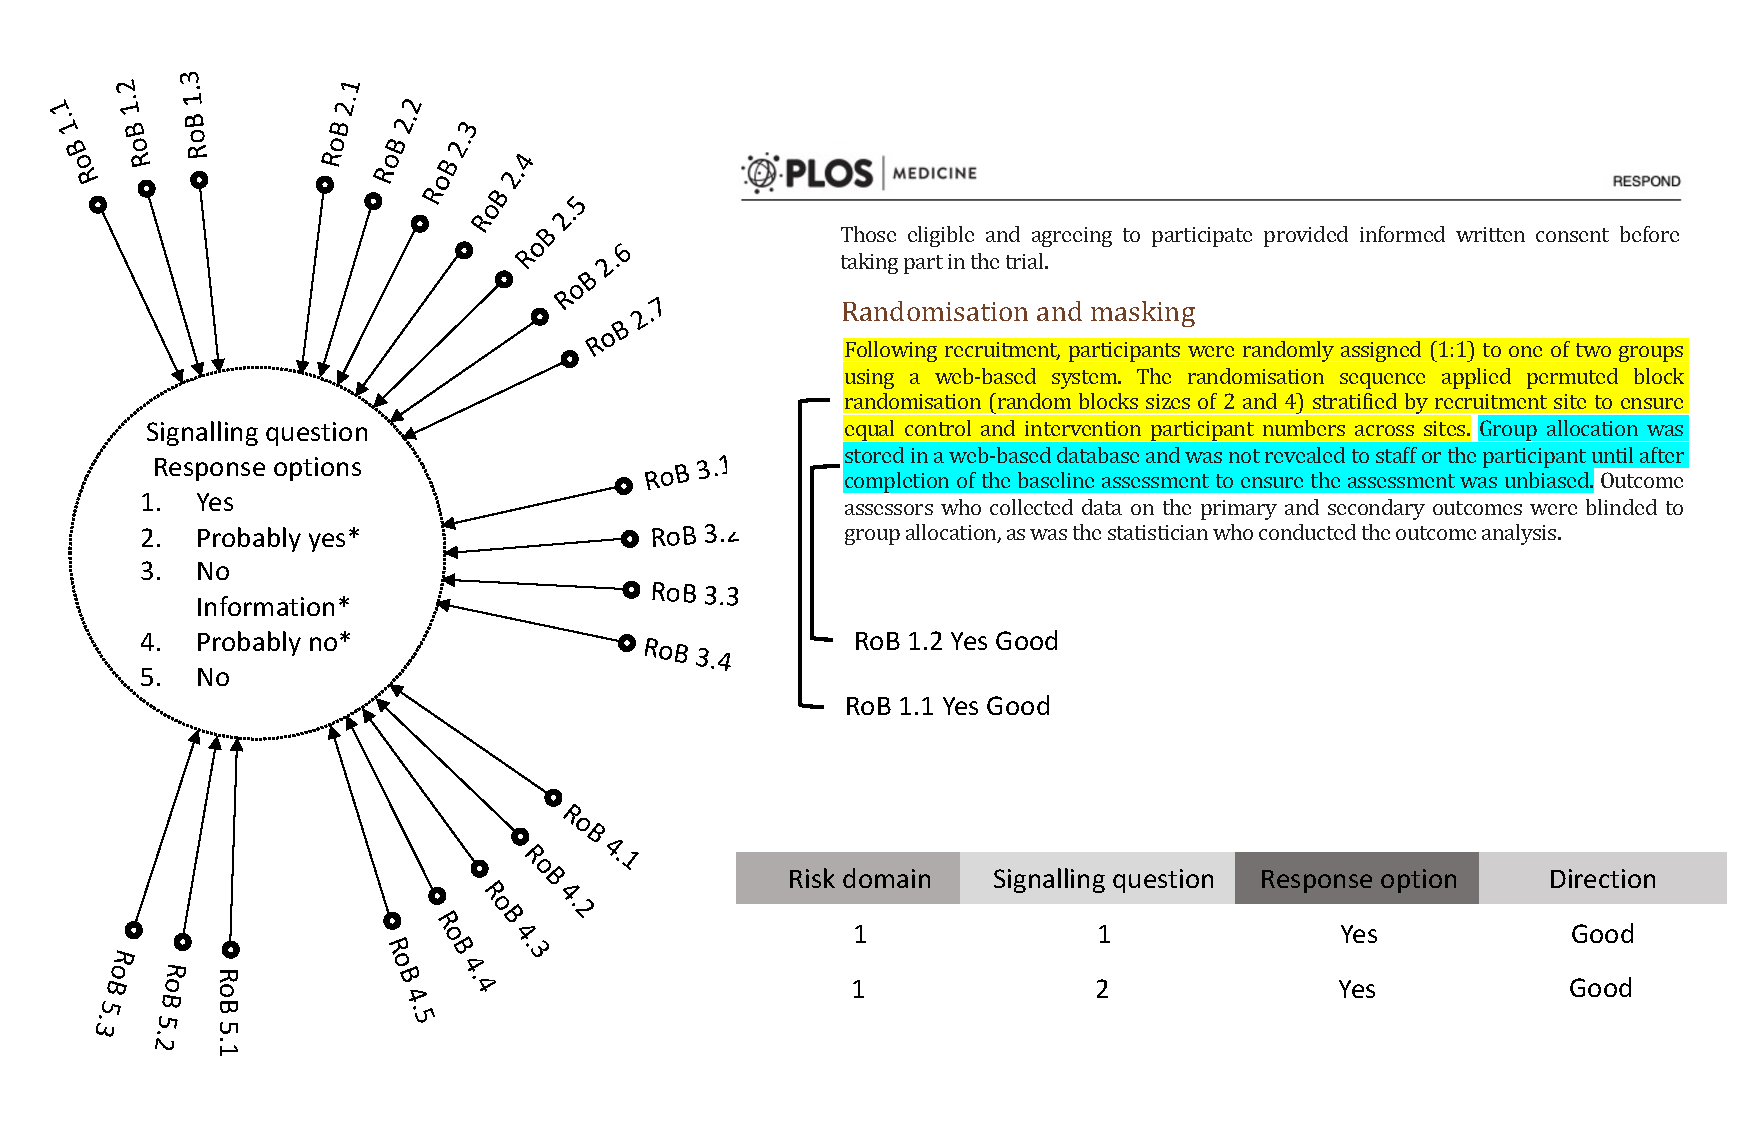
\includegraphics[width=0.99\columnwidth]{figures/annotation_schema.pdf}
    \caption{Our annotation scheme}
    \label{fig:annotationscheme}
\end{figure}
%
%
%



Creating a new annotated corpus involves defining an annotation scheme or adopting an existing one.
To our knowledge the only available annotation scheme for RoB span annotation was presented by~\cite{dhrangadhariya2023first}.
Rather than creating a new scheme, we adapt and enhance their approach by learning from its drawbacks.
Their annotation scheme was directly adapted from the RoB 2 assessment procedure and hence it is imperative to understand the RoB 2 structure to understand the annotation scheme.
RoB 2 divides biases into five risk domains, each loosely corresponding to different parts of the trial design.
Each risk domain decomposes into several signalling questions, each aiming to prompt a relevant response to bias assessment (refer to Table~\ref{tab:robdomains}).


%
%
%
\begin{table*}
 \centering
 %\captionsetup{justification=justified}
   \caption{The table lists down the bias domains as structured in the revised Cochrane RoB assessment tool (RoB 2) and the number of signalling questions (SQ) in each domain.}\label{tab:robdomains}
    \begin{tabular}{llr}
    \toprule[1.0pt]
     Class & Domain & SQ\\
    \midrule[1.0pt]
    RoB 1 & biases arising from the \textbf{randomization process} &  3\\
    RoB 2 & biases due to \textbf{deviations from intended interventions} & 7\\
    RoB 3 & bias due to \textbf{missing outcome data} & 4\\
    RoB 4 & bias in the \textbf{measurement of the outcome} & 5\\
    RoB 5 & bias in the \textbf{selection of the reported result} & 3\\
    \bottomrule[1.0pt]
    \end{tabular}
\end{table*}
%
%
%


The response options are restricted to ``Yes'', ``Probably yes'', ``No'', ``Probably no'', or ``No information''~\cite{sterne2019rob}.
Reviewers assess these signalling questions by examining the factual evidence in the RCT.
For instance, to answer the signalling question ``Was the allocation sequence random?'', the reviewer reads through the study to identify how participants were randomized into intervention groups.
If a well-executed method of randomization is identified, the reviewer answers with ``yes'' (the allocation sequence is random) judging the risk of bias for this signaling question as low risk.
Conversely, if a poorly executed method of randomization is found, the risk of bias is deemed  high risk with response option ``no''.
%Similarly, each signalling question prompts the reviewer to look for a piece(s) of factual evidence in the clinical study to respond with one of the five response options.



In RoB span annotation, we mimic this assessment process by considering evidence text spans in the RCT as the main units of annotation. 
Each span corresponds to answering a signalling question and is annotated with the most informative label. 
The label incorporates information about the signalling question number and the domain it assesses (for the above example, ``1.1'' for the first domain and first signalling question of the domain)
Additionally, the response judgement is incorporated in the label, such as ``1.1 Yes Good'' for a well-executed randomization (see Figure~\ref{fig:annotationscheme}).
Dhrangadhariya \textit{et al.} suggests collapsing the response options ``yes'' and ``probably yes'' into a single ``yes'', and ``no'' and ``probably no'' together into a single ``no'' to increase the inter-annotator agreement (IAA) without altering the final risk domain judgment~\cite{dhrangadhariya2023first}.
As shown in Figure~\ref{fig:flowchart} responding to any signalling question for the risk domain 2 as either ``Probably yes'' or ``Yes'' does not alter the final risk judgment for this domain (low, high, or some concerns).
Therefore, except for some special case signalling questions, we too collapse these response option as suggested.
In summary, the reviewer needs to label the identified text span with the RoB entity along with one of the response options.
In this regard, we have a hierarchical span annotation scheme comprising 22 entities corresponding to the 22 signalling questions, each with typically two response options and two directions (mutually exclusive).
We also remove the ``No Information'' labels since it is meant for the situations where actually no text evidence is found in the RCT to answer a SQ.
However, for selected signalling questions, ``probably yes'', ``probably no'' and ``No Information'' may still be used.
For example, consider that an RCT uses ``...random number generator and sealed envelopes for patient randomization...'', but the trial provided no information on whether the envelop was ``opaque'' or not.
In such situations, ``No Information'' label is acceptable.
%Additionally, it is based on this span, the response judgment option is decided, and therefore even the response judgement information is incorporated in the label.
%Consider the following span is found to answer the above-mentioned signalling question, ``randomized participants using random number generation...'', which is a good randomization procedure and therefore the reviewer responds with ``yes''.
%The label extends the example label to ``1.1 Yes''.
%In addition, a direction is also added to the label, for example, whether it is ``good'' or ``bad.
%In this example, a good randomization ensure low risk for this signalling question and vice versa.
%Adding direction extends the example label to ``1.1 Yes Good''.


%
%
%
\begin{figure}
    \centering
    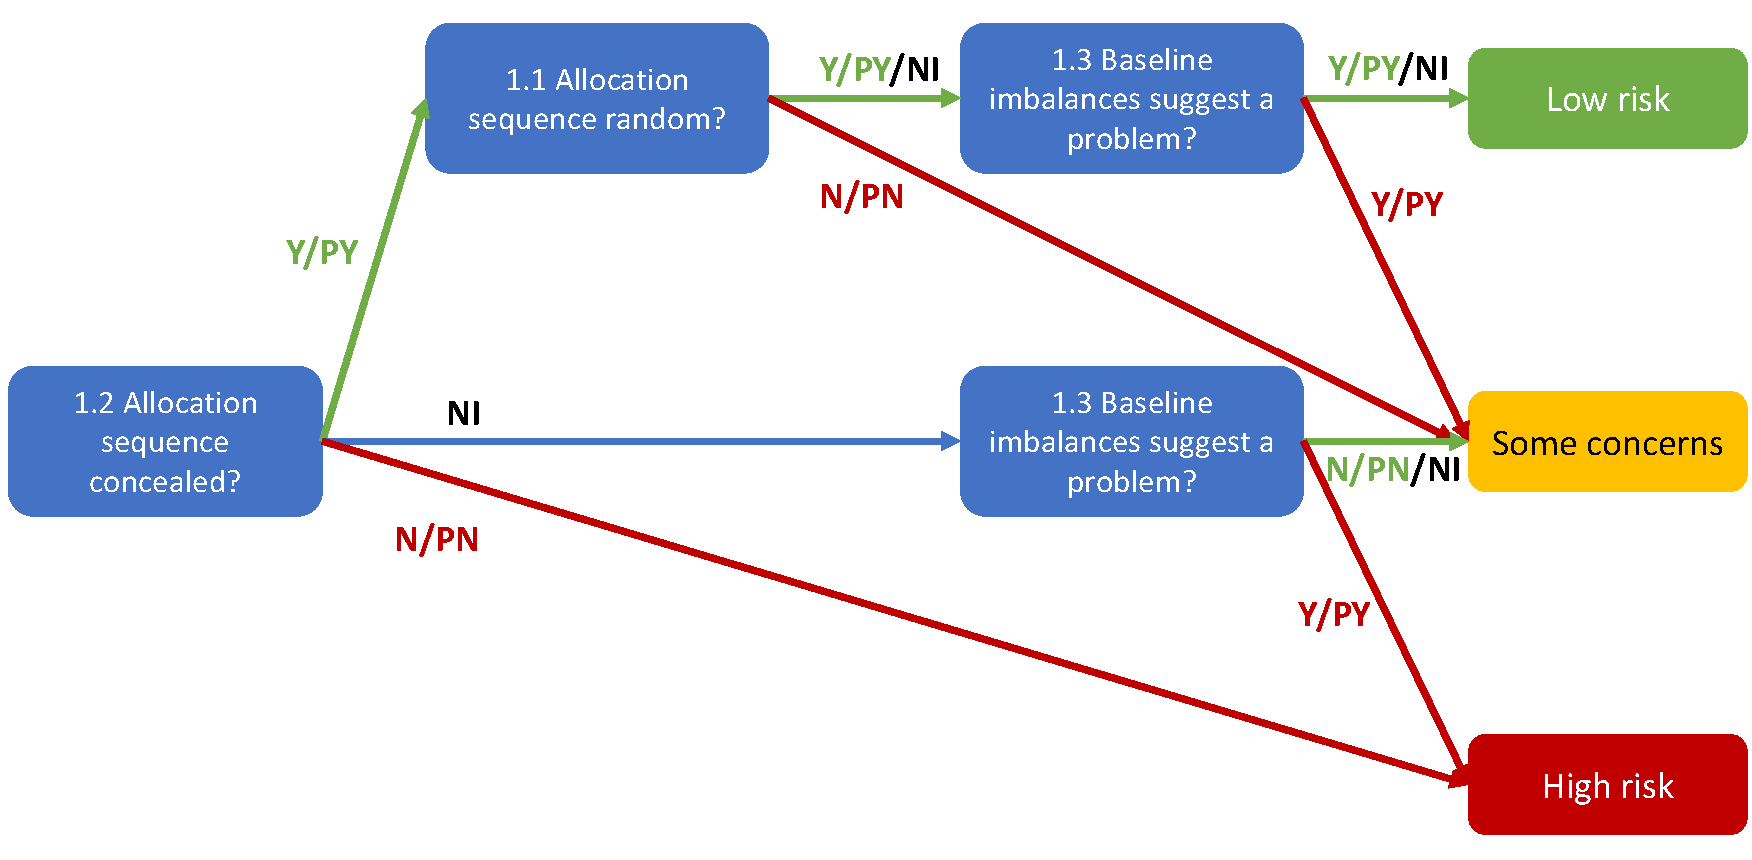
\includegraphics[width=0.80\columnwidth]{figures/flowchart.pdf}
    \caption{Algorithm for suggested judgement of risk of bias arising from the randomization process. The figure is recreated from the revised Cochrane's risk of bias tool (RoB 2).~\cite{sterne2019rob}}
    \label{fig:flowchart}
\end{figure}
%
%
%

%
%
%
\subsection{Data collection}
\label{data}
%
Savović~\textit{et al.} categorized outcome measures as mortality, other objective outcome, or subjective outcome and estimated the associations of bias judgments with intervention effect estimates~\cite{savovic2018association}.
Trials assessing subjective outcomes are more prone to bias, therefore, had we used only one outcome type, we would have limited label types for different risk classes~\cite{page2016empirical}.
In context of RCTs, subjective outcomes are measurements that rely on individuals' perceptions, opinions, or feelings about their own health or well-being.
These outcomes are typically self-reported by the participants in the trial and can be influenced by factors such as  placebo effects, patient expectations, interpretation, and psychological factors.
For example, in a study on rheumatoid arthritis, subjective outcome measures included patient-reported pain ratings~\cite{vollert2020assessment}.
Objective outcomes are measurements that are independent of individual opinions or perceptions and are based on observable and measurable data.
These outcomes are typically collected by trained assessors or through laboratory tests, imaging studies, or other objective methods.
For instance, in a study on peripheral artery disease, objective outcome measures included angiography and molecular imaging to evaluate the effectiveness of cell therapy~\cite{grimaldi2016imaging}.
Mortality outcomes refer to the occurrence of death during the course of the trial.
To ensure these different outcome types are represented in the corpus, we restricted including 17, 17 and 7 RCTs addressing objective, subjective and mortality primary outcomes.
The epidemiology researcher from our team created this 41 RCTs dataset from the domain of physiotherapy and rehabilitation.
PDFs of the full-text RCTs were extracted and each article was collated with its trial protocol from wherever available.
All these RCT PDFs have CC-BY-0 licences~\footnote{\url{https://creativecommons.org/share-your-work/public-domain/cc0/}}.
%
%
%
\subsection{Expert team}
\label{experts}
%
As mentioned earlier, RoB annotation is a complex task that requires specialized expertise.
It's cognitively demanding due to the need to carefully go through the entire full-text of RCTs and identify 22 different bias categories for annotation.
This level of complexity would not be manageable for annotators without expertise in the field.
Our annotation team consisted of two researchers specializing in RoB assessment in physiotherapy and rehabilitation domains, including an epidemiology researcher and an assistant professor in physiotherapy.
With a substantial background in both physiotherapy, advanced statistical methods and experience writing systematic reviews, both experts possesses a deep understanding of the complexities involved in assessing bias risk in research studies.
Two additional physiotherapy experts, a post-doc and a senior PhD student, were a part of developing the visual annotation guidelines.


Additionally, two researchers with expertise in natural language processing (NLP) were involved, one being a computational linguistics professor and the other a PhD student in computer science.
The inclusion of NLP researchers was particularly important because the guidelines and placards they helped create will be utilized to annotate a text corpus, which will serve as a benchmark for the NLP task of RoB span extraction.
%
%
%
\subsection{Guideline development}
\label{guidelines}
%
%
%
%
\begin{figure}
    \centering
    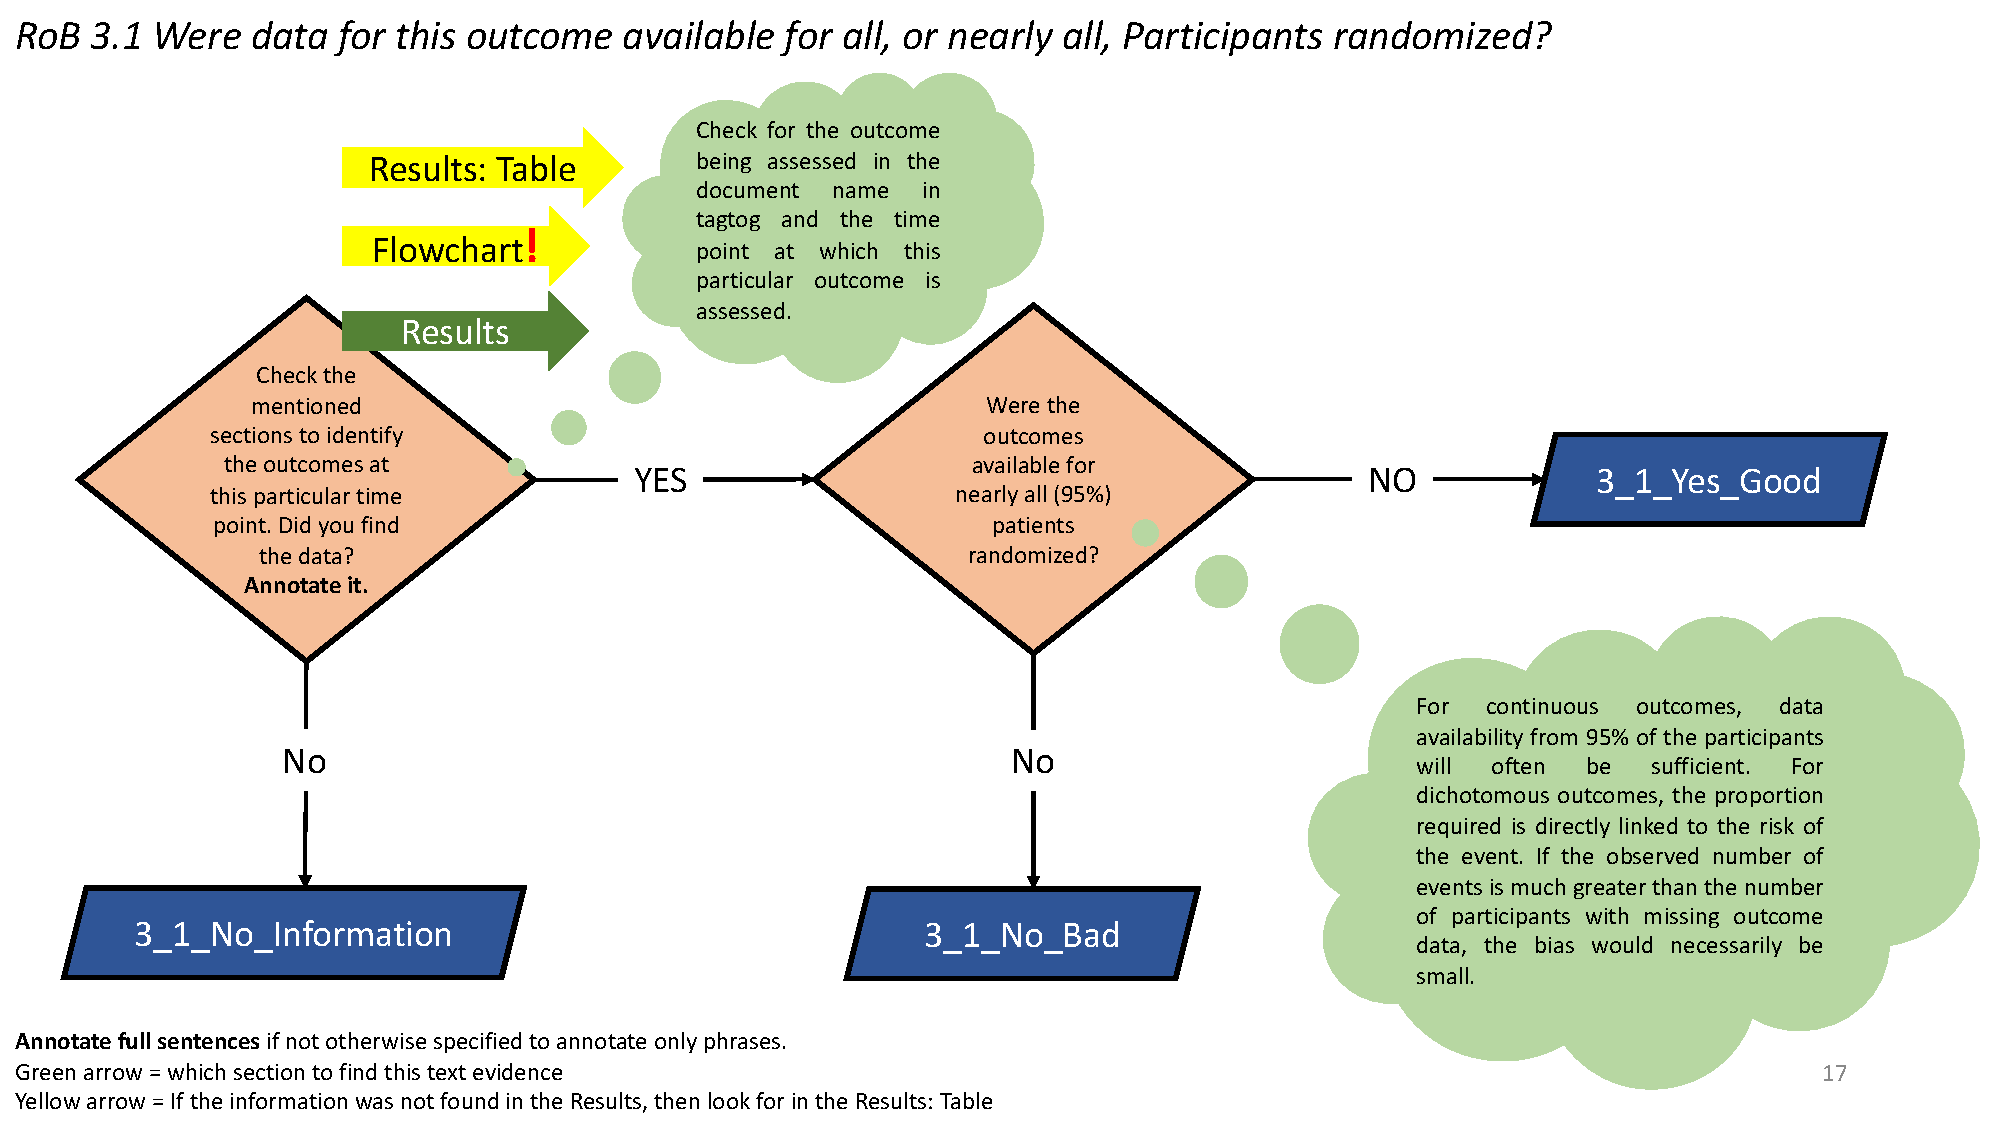
\includegraphics[width=0.80\columnwidth]{figures/placard_3_1.pdf}
    \caption{Sample annotation instruction placard for the signalling question 3.1 designed and adapted using RoB 2 tool.}
    \label{fig:placard}
\end{figure}
%
%
%

RoB 2 guidelines consist of extensive and step-by-step set of instructions that utilize signaling questions, which are detailed in subsection~\ref{met:annot_scheme}.
Even though RoB 2 guidelines are widely used for bias assessment, there have been some research on the reliability of these guidelines.
This reliability concern of RoB 2 has been extensively investigated by Minozzi \textit{et al.}. 
They formulated specific instructions on how to approach and answer the signaling questions of RoB 2.
These instructions, referred to as the Instruction Document (ID), address the subjectivity present in the RoB 2 guidelines and provide clear guidance for the assessment process.
Subjectivity in assessment could potentially result in different evaluators coming to disparate conclusions when analyzing the same trial.
Before implementing the ID, the agreement among four expert RoB assessors was zero, but it improved after adopting the ID.
Several other papers explored subjectivity and reliability of the Cochrane RoB 1.0 and 2 tools~\cite{minozzi2022reliability,da2017effect,loef2022interrater,minozzi2020revised}.
%Anjani: Comments from Roger and Martin about the inherent subjectivity
%The signalling questions are broadly factual but leave room for subjective judgements and aim to facilitate judgements about the risk of bias.


Given the significance of maintaining consistency and reliability among annotators, we undertook the development of precise and clear annotation guidelines.
Working closely with our team of experts, we formatted these guidelines into visual placards.
Each placard takes the form of a flowchart and provides instructions for annotating a single signaling question.
These placards address various facets of RoB 2 subjectivity and the actual process of annotation.
For instance, a common reason for low inter-annotator agreement is when annotators correctly address a bias question but annotate evidence from different parts of the full text. 
To tackle this, our placards restrict annotations for a question to a specific part of the text, such as the Methods section, Results section, Flowchart in the Methods section, etc.
Detailed guidelines and these visual placards are available in the Supplementary material, with an example placard shown in the Figure~\ref{fig:placard}.
These placards also tackle another factor contributing to the low inter-annotator agreement.
For example, while some annotators might annotate an entire paragraph as text evidence to answer a question, others might focus on the most informative portion of the text.
To address this, the placards provide clear guidance on whether annotators should annotate a phrase, a sentence, or a combination of sentences.
%
%
%
\subsection{Annotation}
\label{annotation}
%
%
%
%
\begin{figure}[htb]
    \centering
    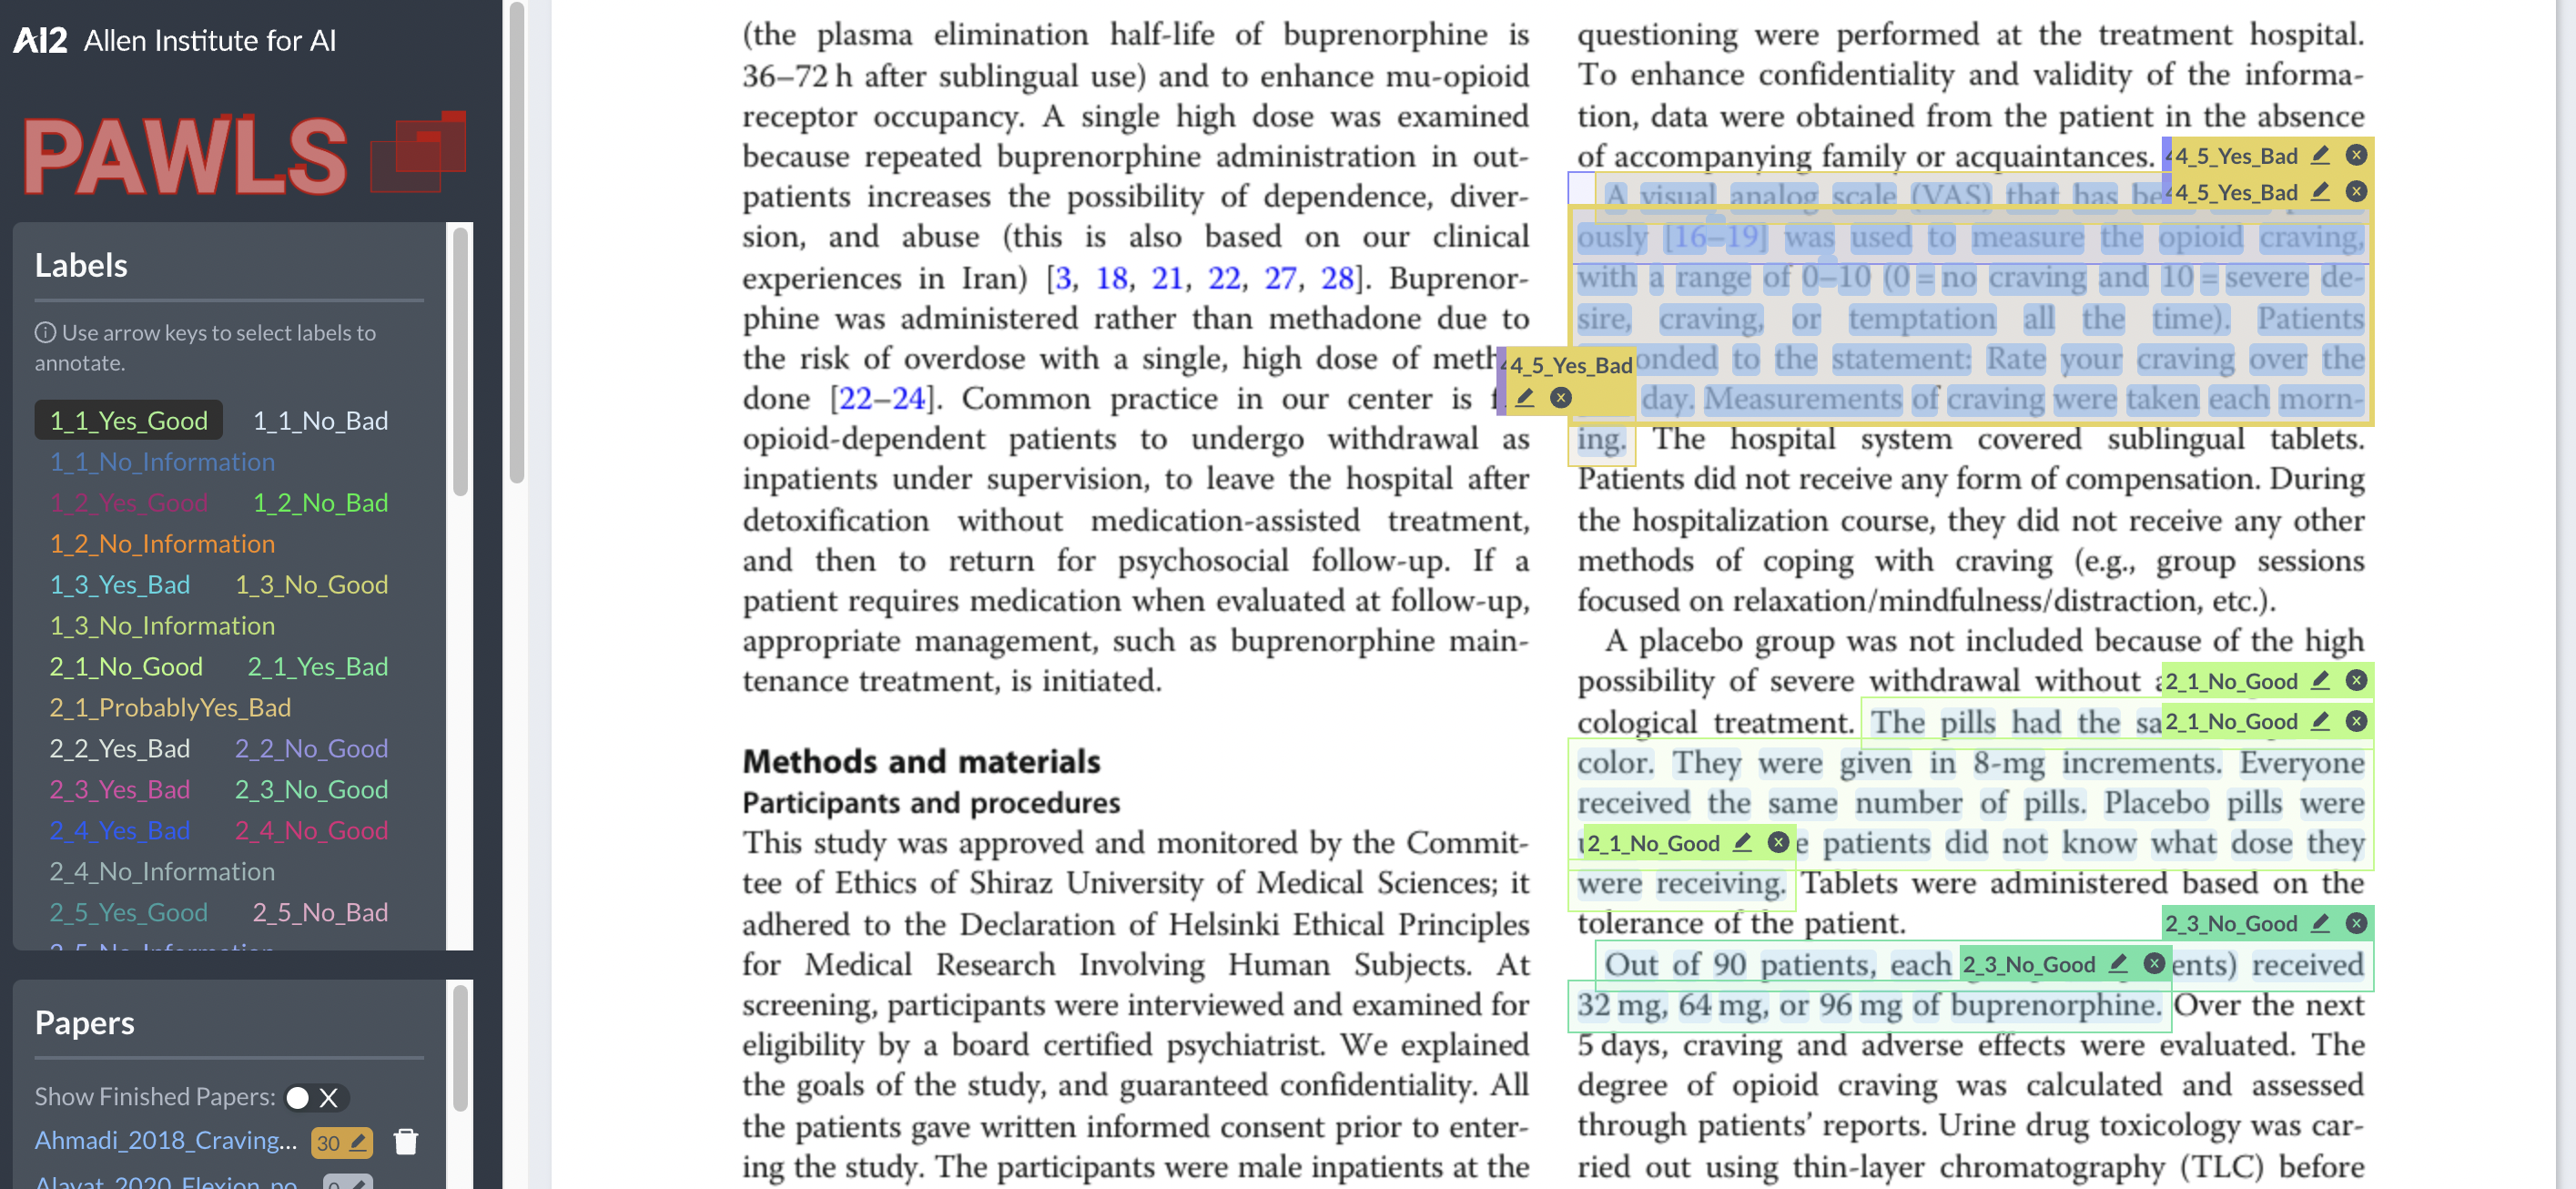
\includegraphics[width=0.80\columnwidth]{figures/pawls_layout.png}
    \caption{A screenshot of PAWLS interface with an example PDF and RoB annotations.}
    \label{fig:pawls}
\end{figure}
%
%
%
For every SQ, the annotators were guided to use the complete RoB 2 guidance document along with visual placards that were developed.
They followed these instructions meticulously, going through each placard's signaling question one by one.
The provided instructions directed the annotators to read specific sections of full-text RCT that needed annotation.
Their task involved identifying and highlighting relevant text related to answering the signaling question.



Tagtog~\footnote{\url{https://www.tagtog.net/}}, a commercial text annotation web application, allows for annotating PDF (Portable Document Format) documents, was used for the annotation~\cite{cejuela2014tagtog}.
Out of the 41 documents, 9 were doubly annotated by two experienced annotators (a epidemiology researcher and an assistant professor) to calculate inter-annotator agreement (IAA) over these documents and the rest were singly annotated by the epidemiology researcher.
After double annotation, we performed conflict resolution to address conflicting annotations, which helped us further calibrate the visual placards.
The conflict resolution was followed by (singly) annotating 31 additional RCTs.


After the annotation of 9 doubly-annotated RCTs, we had to stop using tagtog for certain reasons and switched to the PAWLS~\footnote{\url{https://pawls.apps.allenai.org/}} annotation tool, which allows users to annotate PDFs for free~\cite{neumann2021pawls}.
We chose to annotate PDFs rather than plain text because RCT PDFs have a visual format that will be lost upon converting to text. 
For example the structure pertaining to sections and subsections, tables, and figures makes the annotation task quicker for the annotators and increases annotation quality.
Post annotation, a feedback was taken from all the annotators and the experts involved in formulating the visual placards to gauge the 1) general difficulty, 2) subjectivity and 3) availability of information for bias assessment of each signalling question.
These factors were assessed on the scale of 1-5 with 1 being best and 5 being the worst.
The forms and the responses could be found in the Supplementary material 2. %TODO Anjani: Prepare the supplementary material 
%
%
%
\subsection{Inter-Annotator Agreement}
\label{method:iaa}
%
We report IAA at two levels. 
We check whether the annotators agree on the text spans to answer SQs using the pairwise F1 measure.
Pairwise F1 measure disregards out-of-the-span tokens (unannotated tokens) during agreement calculation and is an ideal measure of annotation reliability for the token-level annotation tasks.
Pairwise F1 calculates the F1 score for each pair of annotators, treating one annotator's labels as the ``true'' labels and the other annotator's labels as the ``predicted'' labels~\cite{deleger2012building,brandsen2020creating}.
We also check how strongly the annotators agree on the response option judgment for each SQ using Cohen's kappa $\kappa$ and compare it with raw percent agreement.
Cohen's kappa $\kappa$ is the standard annotation reliability measure for many classification annotation tasks and is suitable to measure reliability at the response option judgment level.
We interpret both IAA measures as shown in the Table~\ref{tab:iaa_interpret}~\cite{mchugh2012interrater,cohen1960coefficient,landis1977measurement}.
%
%
%
\begin{center}
 \begin{table}[htb]
   \caption{The table details interpretation of pairwise F1-measure (Left), Cohen's kappa (Middle) and Observed or raw agreement (Left)}\label{tab:iaa_interpret}
 \centering
    \begin{tabular}{lr|lr|lr}
    \toprule[1.0pt]
    \multicolumn{2}{c|}{F1 Measure} & \multicolumn{2}{c|}{Cohen's Kappa}& \multicolumn{2}{c}{Raw Agreement}  \\ 
    interpretation & range & interpretation & range & interpretation & range \\ 
    \midrule[1.0pt]
        Poor & 0-0.99 &  No agreement& $\leq$ 0 & None & 0 \\ 
        Slight & 1 - 20.99 &  None to slight agreement & 0-0.20 & Very low & 1-10\% \\ 
        Fair & 21 - 40.99 &  Minimal & 0.21-0.39 & Low & 11-30\% \\ 
        Good & 41 - 60.99 & Weak & 0.40-0.59 & Moderate & 31-50\% \\ 
        Substantial & 61 - 80.99 & Moderate & 0.60-0.79 & High & 51-70\% \\ 
        Almost perfect & 81 - 99.99 & Strong & 0.80-0.90 & Very high & 71-90\% \\ 
        Perfect & 100 & Almost Perfect & $\geq$ 0.90 & Perfect & $>$90\% \\ 
         & & Perfect & 1.0 \\ 
    \bottomrule[1.0pt]
    \end{tabular}
 \end{table}   
\end{center}
%
%
%
\subsection{LLM evaluation}
\label{method:llm}
%
Our annotation guidelines and annotations were adapted for benchmarking classical supervised machine learning approaches and not LLMs.
So even though we were annotating PDFs, we had to restrict a lot of annotations based on the assumption that PDF will be converted into text via OCR (optical character recognition) losing its structure of tables and figures, which anyway a classical ML model could not use without extensive modifications~\cite{li2019figure,li2023uttsr}.
However, recent advancements with LLMs that encode vast amounts of knowledge offers a better alternative made us rethink the evaluation.
The bar for clinical applications is high and it is imperative to evaluate these models for the more challenging clinical tasks like RoB text span extraction~\cite{singhal2023large}.
Additionally, the tools like ChatPDF~\footnote{\url{https://www.chatpdf.com/}} allows direct interaction between GPT-3.5 (Generative Pretrained Model) and PDFs, negating the clumsy PDF to text conversion.
Therefore, we consider it essential to evaluate LLMs instead of forcefully adapting the evaluation to a classical ML problem.
We formulated the task as a zero-shot RoB text span extraction task.
This was to gauge whether GPT-3.5 encodes knowledge related to assessing trial biases.
We will use simple prompt constructs of the structure ``Answer the \{\textit{signalling question}\} + Action item to extract sentence supporting the answer''.
Consider the following example.

\begin{quote}
\itshape Example prompt: Question 4.3 Were outcome assessors aware of the intervention received by study participants? Provide an answer and extract the supporting sentences that you write your answer based on. Extract the sentences in JSON~\footnote{JSON = JavaScript Object Notation}.
\end{quote}

The prompt serves two purposes for evaluating LLMs for correctness.
ChatPDF is tasked with 1) answering the SQ with a response option (the judgment), and 2) extract the text evidence to support their answer.
When answering a question, ChatPDF finds the most relevant paragraphs from the PDF and uses the ChatGPT API from OpenAI to generate an answer.
ChatPDF employs GPT (Generative Pretrained Transformer) 3.5.
ChatPDF is required to do the same task as human annotators and they will be evaluated on the basis of correctness of the answer.
If ChatPDF answer corresponds to response option selected by the expert annotator, it is considered a correct answer for that SQ. 
If the text extracted by LLMs as evidence for answering the SQ fuzzy matches the text selected by the expert annotator, it is considered a correct answer.
Both of these skills will be evaluated using a raw or observed agreement metrics $P_{O} (Extraction)$  for measuring agreement over extraction and $P_{O} (Response)$ for measuring agreement over response judgments and interpreted as per Table~\ref{tab:iaa_interpret}. 
Observed agreement is essentially the number of documents for a RoB SQ where ChatPDFs responses align with those of the human expert, divided by the total number of documents assessed~\cite{artstein2017inter}.
In several instances, there was no information found by the expert annotator from the RCT to answer a question. 
For such instances, if ChatPDF correctly identifies the absence of relevant information to answer a question, it is considered a correct response.
It's important to highlight that the evaluation framework is designed solely to measure the agreement of the answers between ChatPDF and the expert.
This evaluation was manually conducted by a bias assessment assessor for 10 out of the 41 RCTs.
%
%
%
\section{Results}
\label{sec:results}
%
This section outlines the annotated dataset, presents the inter-annotator agreement findings, and the outcomes of the LLM evaluation.
%
%
%
\subsection{The corpus}
\label{subsec:corpus}
%
In this section, we provide key statistical information about the annotations in our corpus.
The histogram in Figure \ref{fig:ann_counts} shows a visual representation of the absolute counts of annotations (tokens) for each of the RoB signaling questions.
SQ 1.3 had disproportionately higher number of annotated tokens, while for all other SQs, the number of annotated tokens remained consistently below 2000 across the entire corpus.
The only exception to this trend was for SQ 3.1 which had slightly more than 2000 annotated tokens.
There were only 25 annotated tokens for SQ 2.4 ``Were these deviations likely to have affected the outcome?''.


Table~\ref{table:stats} lists down essential information on the absolute and average annotation lengths for each RoB SQ along with the total number of documents the annotations were identified from.
Annotations from risk domain one (biases arising due to randomization process) were found in an average of 35 of the 41 documents, while information related to answering the other risk questions was available only in a small subset of the total annotated RCTs, as also depicted in Figure~\ref{fig:rob_information}.
Notably, SQs 2.2, 2.6, 3.1, 4.3, and 4.4 stood out as exceptions, with information available in more than 50\% of the annotated documents.
The figure highlights that, for most RoB questions, no information was available (indicated by yellow bars) for both answering the question and making a judgment about the bias level. 
In cases where information was available, bias tended to be low, as indicated by the prevalence of green bars. 
However, exceptions were observed, such as in SQs 2.1, 2.2, 3.1, 4.3, and 4.4, where bias was high, as indicated by the prevalence of red bars.
Check the Supplementary material for the references of included studies.
%
%
%
\begin{figure}[htb]
    \centering
    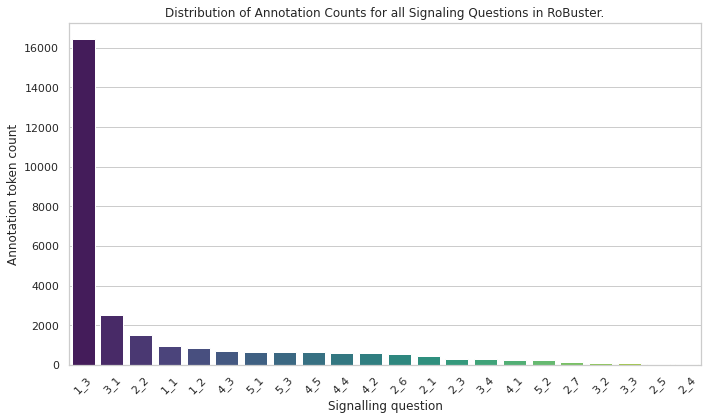
\includegraphics[width=0.90\columnwidth]{figures/annot_counts.png}
    \caption{Total number of token annotations for each RoB signalling question.}
    \label{fig:ann_counts}
\end{figure}
%
%
%

%
%
%
\begin{table}[htb]
    \centering
    \caption{General statistics for the annotated corpus: This table provides an overview of the annotated corpus, including the total number of annotated tokens, the average length of token sequences, and the number of documents in which annotations were identified, out of a total of 41 annotated documents.}
    \label{table:stats}
    \begin{tabular}{crrr}
    \toprule[1.0pt]
        Signalling question & Total tokens & Average length & Total documents \\
    \midrule[1.0pt]
        \multicolumn{4}{c}{Domain 1: Biases arising from the randomization process} \\
        \hline
        RoB1.1 & 960 & 32 & 30 \\
        RoB1.2 & 838 & 24.65 & 34 \\
        RoB1.3 & 16446 & 411.15 & 40 \\
        \hline
        \multicolumn{4}{c}{Domain 2: Biases due to deviations from intended interventions} \\
        \hline
        RoB2.1 & 455 & 32.5 & 14 \\
        RoB2.2 & 1502 & 55.63 & 27 \\
        RoB2.3 & 282 & 56.4 & 5 \\
        RoB2.4 & 25 & 25 & 1 \\
        RoB2.5 & 58 & 29 & 2 \\
        RoB2.6 & 544 & 20.92 & 26 \\
        RoB2.7 & 126 & 25.2 & 5 \\
        \hline
        \multicolumn{4}{c}{Domain 3: Bias due to missing outcome data} \\
        \hline
        RoB3.1 & 2529 & 74.38 & 34 \\
        RoB3.2 & 103 & 34.33 & 3 \\
        RoB3.3 & 75 & 15 & 5 \\
        RoB3.4 & 276 & 21.23 & 13 \\
        \hline
        \multicolumn{4}{c}{Domain 4: Bias in the measurement of the outcome} \\
        \hline
        RoB4.1 & 240 & 24 & 10 \\
        RoB4.2 & 572 & 33.65 & 17 \\
        RoB4.3 & 698 & 30.35 & 23 \\
        RoB4.4 & 585 & 27.86 & 21 \\
        RoB4.5 & 622 & 41.47 & 15 \\
        \hline
        \multicolumn{4}{c}{Domain 5: Bias in the selection of the reported result} \\
        \hline
        RoB5.1 & 628 & 69.78 & 9 \\
        RoB5.2 & 235 & 19.58 & 12 \\
        RoB5.3 & 628 & 89.71 & 7 \\
    \bottomrule[1.0pt]
    \end{tabular}
\end{table}
%
%
%

%
%
%
\begin{figure}[htb]
    \centering
    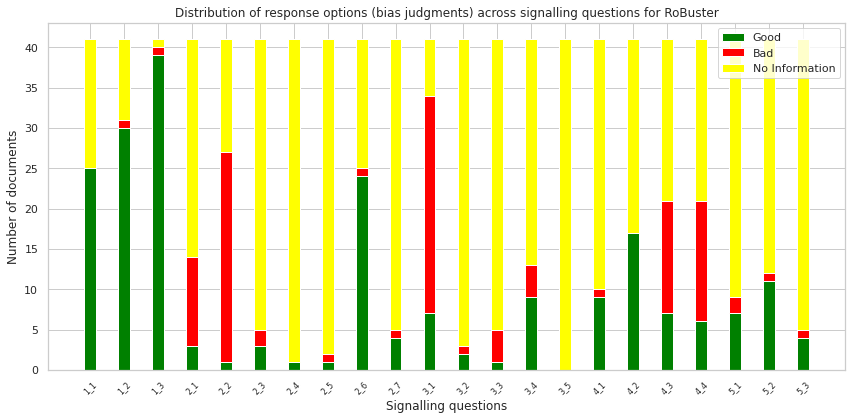
\includegraphics[width=0.90\columnwidth]{figures/bias_chart.png}
    \caption{Distribution of bias judgment across RoB signalling questions in RoBuster.}
    \label{fig:rob_information}
\end{figure}
%
%
%

%
%
%
\subsection{Inter-annotator agreement}
\label{result:iaa}
%
Table~\ref{tab:IAA_sq} illustrates the levels of F1-measure (inter-annotator agreement) between the two annotators, both before and after the development of the visual placards.
The IAA scores before and after the guideline improvement were calculated on a different set of documents.
The average overall F1-measure agreement across the corpus exhibited a modest 10.87\% agreement before the introduction of visual placards. Following the implementation, this agreement increased significantly by 17.14 percentage points, reaching a fair 28.01\%.
The increase in agreement was visible at the domain level.
The F1-measure agreement for the ``randomization'' domain 1 doubled from a poor 31.72 to a substantial 63.30.
for the ``deviations from intended interventions'' domain 2, the agreement increased from a slight 12.76 to a fair 27.02.
In the case of the ``missing outcomes'' domain 3, the agreement rose from 5.89 to 9.92, although it remained within the slight agreement category for this domain. 
For the ``missing outcome measurement'' domain (domain 4) the agreement increased from 4.072 to 17.29.
The agreement before the placard development was none (0) and it increased to slight (16.49) for the ``selection of reported results'' domain 5.



Improvements in agreement were observed at individual signaling questions level too, with considerable gains exceeding 50\% points for signaling questions 1.3, 2.1, 4.1, and 4.4.
The IAA between the two reference annotators for a total of 11 out of 22 questions remained zero both before and after the guideline development.
Only for two signalling questions, 4.4 and 5.2, did the guideline improvement raise the IAA from zero to 56.25 and 49.49 respectively.
However, for signaling questions 2.3 and 2.7, the agreement experienced a modest decline of 5.42 and 6.52, reaching zero after the guideline development.
For the SQ 1.2, the F1-measure dropped by 6.28\% points making it a drop in agreement for three signalling questions.
Inferring from the table~\ref{tab:iaa_interpret} and table~\ref{tab:IAA_sq}, annotators for 11 of the 22 signalling questions had a poor agreement, three of the 22 questions had a fair agreement, four out of the 22 questions had a good agreement and two out of the 22 questions had a substantial agreement while only two of the 22 questions had an almost perfect agreement of beyond 81 IAA points.
As expected, none of the SQ annotations had a perfect IAA of 100.
%
%
%
\begin{table}[htb]
    \caption{F1-Measure (Inter-Annotator Agreement) Comparison Before and After Visual Placard Development: This table displays the F1-Measure at the text span answer level before and after the development of visual placards. The change in F1-Measure is presented in terms of absolute IAA points.}
    \label{tab:IAA_sq}
    \centering
    \begin{tabular}{crrr}
    \toprule[1.0pt]
         & \multicolumn{2}{c}{F1-measure IAA} & \\
        Signalling question & before guideline improvement & after guidelines improvement & change \\
    \midrule[1.0pt]
        \multicolumn{4}{c}{Domain 1: Biases arising from the randomization process} \\
        \hline
        RoB 1\_1 & 24.44 & 55.02 & +30.58 \\ 
        RoB 1\_2 & 50.28 & 44 & -6.28 \\ 
        RoB 1\_3 & 20.44 & 90.9 & +70.46 \\
        \hline
        \multicolumn{4}{c}{Domain 2: Biases due to deviations from intended interventions} \\
        \hline
        RoB 2\_1 & 1.34 & 67.26 & +65.92 \\ 
        RoB 2\_2 & 7.23 & 38.66 & +31.43 \\ 
        RoB 2\_3 & 5.42 & 0 & -5.42 \\ 
        RoB 2\_4 & - & 0 & 0 \\ 
        RoB 2\_5 & 0 & 0 & 0 \\ 
        RoB 2\_6 & 68.85 & 83.25 & +14.4 \\ 
        RoB 2\_7 & 6.52 & 0 & -6.52 \\ 
        \hline
        \multicolumn{4}{c}{Domain 3: Bias due to missing outcome data} \\
        \hline
        RoB 3\_1 & 23.57 & 39.68 & +16.11 \\ 
        RoB 3\_2 & 0 & 0 & 0 \\ 
        RoB 3\_3 & 0 & 0 & 0 \\ 
        RoB 3\_4 & 0 & 0 & 0 \\ 
        \hline
        \multicolumn{4}{c}{Domain 4: Bias in the measurement of the outcome} \\
        \hline
        RoB 4\_1 & 6.51 & 61.71 & +55.2 \\ 
        RoB 4\_2 & 0 & 0 & 0 \\ 
        RoB 4\_3 & 13.85 & 30.21 & +16.36 \\ 
        RoB 4\_4 & 0 & 56.25 & +56.25 \\ 
        RoB 4\_5 & 0 & 0 & 0 \\ 
        \hline
        \multicolumn{4}{c}{Domain 5: Bias in the selection of the reported result} \\
        \hline
        RoB 5\_1 & 0 & 0 & 0 \\ 
        RoB 5\_2 & 0 & 49.49 & +49.49 \\ 
        RoB 5\_3 & 0 & 0 & 0 \\
    \bottomrule[1.0pt]
    \end{tabular}
\end{table}
%
%
%

We present the Cohen's Kappa ($\kappa$) scores and observed or raw agreement in Table~\ref{tab:IAA_response}~\cite{mchugh2012interrater} which measure agreement at the SQ response judgment level.
Additionally, we provide the percentage of these agreements that stems from the ``No Information'' judgments.
Cohen's kappa quantifies the extent to which two raters' classifications agree beyond what would be expected by chance.
The overall $\kappa$ agreement between the raters stands at a weak 0.5187 IAA.
The average $\kappa$ agreement for randomization domain was 0.27 IAA which is a minimal agreement.
For the ``deviations due to intended interventions'', there was minimal agreement of 0.33 IAA and for the ``due to missing outcome data'' domain there was a better though weak agreement of 0.494 IAA.
The last two domains ``measurement of the outcome'' and ``selection of the reported result'' had agreements 0.0996 IAA and -0.0036 IAA interpreted as zero and negative.



The highest $\kappa$ agreement of 1.0 is observed for SQ 2.6.
It is, however, important to note that more than half of this agreement arises from the assumed ``No Information'' judgments.
For the remaining signaling questions, we do not find any instances of either almost perfect or strong agreement.
Agreements for SQs 2.1, 3.1, and 4.3 fall within the moderate agreement category (ranging from 0.60 to 0.80 IAA), with no substantial agreement originating from the ``No Information'' judgments for either of them.
In contrast, six of the 22 signaling questions (2.4, 2.5, 4.1, 4.2, 4.5, and 5.3) exhibit agreement worse than what would be expected by chance, and considerable percentage of them stems from ``No Information'' judgments.
The bias questions 1.3, 2.3 and 5.1 show zero $\kappa$ agreement and variable observed agreement.



%
%
%
\begin{table}[]
    \caption{Cohen's Kappa $\kappa$ and raw agreement between annotator pairs for agreement at the response option level for each signalling question.}
    \label{tab:IAA_response}
    \begin{tabular}{crrr}
    \toprule[1.0pt]
        Signalling question & $\kappa$ agreement & Raw agreement & Contribution from ``No Information'' \\
    \midrule[1.0pt]
        \multicolumn{4}{c}{Biases arising from the randomization process} \\
        \hline
        RoB 1\_1 & 0.571 & 88.9\%  & 22.22\% \\
        RoB 1\_2 & 0.25 & 66.7\%  & 33.33\% \\
        RoB 1\_3 & 0 & 77.8\%  & 11.11\% \\
        \hline 
        \multicolumn{4}{c}{Biases due to deviations from intended interventions} \\
        \hline
        RoB 2\_1 & 0.727 & 77.8\%  & 5.55\% \\
        RoB 2\_2 & 0.449 & 66.7\%  & 38.88\% \\
        RoB 2\_3 & 0 & 66.7 & 77.77\% \\
        RoB 2\_4 & -0.125 & 77.8\%  & 88.88\% \\
        RoB 2\_5 & -0.08 & 77.8\%  & 83.33\% \\
        RoB 2\_6 & 1 & 100\%  & 55.55\% \\
        RoB 2\_7 & 0.357 & 77.8\%  & 77.77\% \\
        \hline
        \multicolumn{4}{c}{Bias due to missing outcome data} \\
        \hline
        RoB 3\_1 & 0.75 & 88.9\%  & 11.11\% \\
        RoB 3\_2 & - & 1 & 100\% \\
        RoB 3\_3 & 0.20.6 & 33.3\%  & 55.55\% \\
        RoB 3\_4 & 0.52.6 & 55.6\%  & 33.33\% \\
        \hline
        \multicolumn{4}{c}{Bias in the measurement of the outcome} \\
        \hline
        RoB 4\_1 & -0.125 & 77.8\%  & 11.11\% \\
        RoB 4\_2 & -0.235 & 22.2\%  & 38.88\% \\
        RoB 4\_3 & 0.63 & 77.8\%  & 27.77\% \\
        RoB 4\_4 & 0.308 & 44.4\%  & 22.22\% \\
        RoB 4\_5 & -0.08 & 33.3\%  & 66.66\% \\
        \hline
        \multicolumn{4}{c}{Bias in the selection of the reported result} \\
        \hline
        RoB 5\_1 & 0 & 22.2\%  & 61.11\% \\
        RoB 5\_2 & 0.143 & 66.7\%  & 22.22\% \\
        RoB 5\_3 & -0.154 & 55.6\%  & 72.22\% \\
    \bottomrule[1.0pt]
    \end{tabular}
\end{table}

%
%
%
\subsection{LLM evaluation}
%
In the Table~\ref{table:LLM_eval}, we report the observed or raw agreement between LLMs and the expert in extracting and responding to the SQs over a subset (n=10) of RoBuster~\ref{method:llm}.
For the first risk domain, ChatGPT has an high $P_{O} (Extraction)$ and $P_{O} (Response)$ agreements (66.6\% and 55.3\% IAA respectively) with experts with none of these agreements coming from ``No Information'' responses.
These agreements for the the second domain are even higher 64.28\% and 60\% respectively, but 40\% of these agreements emanate from ``No Information'' responses.
\textcolor{blue}{The results for risk domain 3, 4 and 5 remain.}

%
%
%
\begin{table}[htb]
    \caption{LLM accuracy}
    \label{table:LLM_eval}
    \centering
    \begin{tabular}{crrr}
    \toprule[1.0pt]
     & \multicolumn{2}{c}{Observed Agreement $P_{O}$} \\
        SQ & $P_{O} (Extraction)$ & $P_{O} (Response)$ & ``No Information'' \\ 
    \midrule[1.0pt]
        \multicolumn{4}{c}{Biases arising from the randomization process} \\
        \hline
        RoB 1\_1 & 90\% & 70\% & 0\% \\ 
        RoB 1\_2 & 70\% & 60\% & 0\% \\ 
        RoB 1\_3 & 40\% & 30\% & 0\% \\ 
        \hline
        \multicolumn{4}{c}{Biases due to deviations from intended interventions} \\
        \hline
        RoB 2\_1 & 50\% & 40\% & 0\% \\
        RoB 2\_2 & 30\% & 30\% & 10\% \\ 
        RoB 2\_3 & 60\% & 60\% & 50\% \\ 
        RoB 2\_4 & 90\% & 90\% & 100\% \\ 
        RoB 2\_5 & 90\% & 90\% & 100\% \\ 
        RoB 2\_6 & 80\% & 50\% & 10\% \\ 
        RoB 2\_7 & 50\% & 60\% & 40\% \\
        \hline
        \multicolumn{4}{c}{Bias due to missing outcome data} \\
        \hline
        RoB 3\_1 & & & \\ 
        RoB 3\_2 & & & \\ 
        RoB 3\_3 & & & \\ 
        RoB 3\_4 & & & \\ 
        \hline
        \multicolumn{4}{c}{Bias in the measurement of the outcome} \\
        \hline
        RoB 4\_1 & & & \\ 
        RoB 4\_2 & & & \\ 
        RoB 4\_3 & & & \\ 
        RoB 4\_4 & & & \\ 
        RoB 4\_5 & & & \\ 
        \hline
        \multicolumn{4}{c}{Bias in the selection of the reported result} \\
        \hline
        RoB 5\_1 & & & \\ 
        RoB 5\_2 & & & \\ 
        RoB 5\_3 & & & \\
    \bottomrule[1.0pt]
    \end{tabular}
\end{table}
%
%
%
\section{Discussion}
\label{sec:discussion}
%
%
%
\subsection{The Corpus}
\label{disc:corpus}
%
The immediate points we noticed in the Figure~\ref{fig:ann_counts} was that SQ 1.3 had a disproportionately higher number of annotated tokens (n=16,446) while the remaining signal questions had fewer than 2600 tokens each annotated.
The reason behind this is that the answer to SQ 1.3 is found in the table detailing baseline patient characteristics of the intervention groups.
To ensure good annotator agreement, instructions on visual placards directed annotators to label the entire table, leading to a higher count of annotated tokens for this question.
For the rest of the question, it is the availability of detailed description on the study design, methods and results that could impact the amount of tokens annotated and also the ease of bias assessment.
The more information a study provided, the easier it is to evaluate a bias question.
Some studies tend to not report key details making it tougher to assess certain bias questions.
Feedback received indicates that for signal questions with fewer than 100 annotated tokens, annotators consistently rated the availability of information to answer those questions as either ``low'' or ``very low''.
In contrast, for the top five signal questions shown in Figure~\ref{fig:ann_counts}, both annotators consistently rated the availability of information as ``high'' and ``normal''.
Though it is important to interpret this qualitative feedback with caution, as annotator ratings are influenced by the number and types of RCTs they annotated.
Annotator who reviewed a greater number of documents in RoBuster experienced that it was more difficult to assess certain questions and the availability of information was lower than the other annotator who annotated fewer documents.
%
%
%
\subsection{Inter-Annotator Agreement}
\label{disc:iaa}
%
\subsubsection{Text span agreement}
\label{disc:f1}
%
% Were the visual placards effective?
F1-measure agreement was calculated before and after visual placard development.
Using the visual placards improves the F1 agreement for choosing the RCT text spans for 10 of the 22 SQs showing their utility in aiding decision making.
% For which SQs did the agreement increase and why?
SQ 1.3 had the highest increase of 70.46 F1 IAA points thanks to the visual placards requesting to look for the text evidence to answer this question first priority in the table recording patient characteristics and instructs to mark the entire table along with the table caption.
Before the development of these placards, annotators would only mark a portion of the table to answer this question. 
The specific text selected by an annotator depended on which part of the table text they noticed first as potentially indicating bias given any of the listed patient characteristics could show imbalances between the groups.
This variability in selection led to lower F1 agreement on this SQ, which has significantly improved with the introduction of the placards.
SQ 1.1 recorded an improvement of more than 30 F1 IAA points thanks to the placards instructing the annotators to mark the text evidence in the Methods section as a priority. 
The evidence to answer the SQ 1.1 could be found in both abstract and the methods section and prior to placard development, the annotators variably marked the answer to this question leading to a lower agreement.
We restricted annotating this text in the methods section in the visual placards because a more detailed textual description is found in this section and consequently saw an increase in agreement by 30.58 F1 IAA.
These improvements were also the reason for an increased agreement for the SQs 2.1 and 2.2.
For SQ 2.1, there was a remarkable increase of 67.26 IAA points.
This can be attributed to the comprehensive instructions provided by the visual placards, which instruct annotators to specifically identify and label text descriptions related to intervention administration and placebo administration.
Prior to the placard development the annotators were inconsistently annotating either the description of intervention administration or placebo administration, leading to lower agreement.


% Why do some RoB questions have more annotations compared to the other? Does it mean papers have more information on certain aspects compared to the other questions?
%How did the annotators perceive the difficulty of each signalling question? -> Make a scale
% Why were agreements on certain questions zero?
While the agreement drastically increased for certain SQs, for other questions it remained zero.
These outcomes align with the feedback forms' findings.
Almost all the RoB questions where the IAA between the annotators was zero (2.3, 2.4, 2.5, 2.7, 3.2, 3.3, 3.4, 4.2, 4.5, 5.1, 5.3) consistently received remarks from one or both annotators regarding their higher subjectivity, difficulty in assessment, and lower availability of information for evaluation.
The poor agreement hence can be well assumed to caused by the subjectivity of the signalling questions, lack of information to annotate in the RCT, theoretical nature of the signalling questions and the overall complex process of analysing trials.
% TODO: Why was the agreement for question 2.3, 2.4 and 2.5 zero?
Also, we did not have F1 IAA score on SQ 2.4 because, while two out of the nine annotations had annotations for 2.4, these annotations were made by only one of the annotators and not by both annotators lading to no agreement at the span level.


% Theoretical nature of the signalling questions and zero agreement?
A lower IAA score could also be attributed to the theoretical nature of certain signalling question.
Consider the questions 3.4 and 4.5.
The SQ 3.4 in RoB assesses the ``likelihood'' that missing data on outcome measures is related to the true values of those outcomes. 
It evaluates the risk of bias associated with missing outcome data.
This question is theoretical and depends on the assessment of whether there could be a relationship between the outcome missingness and the true values of the outcomes.
The same applies to SQ 4.5, which relies on the results of SQ 4.4.
It seeks to gauge the ``likelihood'' that the assessment of the outcome was influenced by knowledge of whether the intervention was received or not.
Such ``theoretical'' questions require making judgments that rely on hypothetical scenarios rather than direct observations or concrete evidence leading to higher subjectivity of assessment results.
As these questions pertain to aspects of study design, conduct, or reporting that may not be explicitly addressed in the trial documentation these questions also suffer from a lack of information that could be annotated in a trial.
Availability of annotations is also important to train and evaluate ML models and therefore determine the utility of a corpus.
To ensure some kind of annotations are always available to make a judgment , we instruct annotators to annotate the outcome and outcome measurement descriptions in the paper for these questions.


% Were certain RoB questions more subjective than the others?
There were certain aspects where question subjectivity might have led to low agreement score.
For example, for the SQ 2.4, it is asked whether deviations from the intended intervention could have affected the outcome.
Assessing whether deviations could have affected outcomes requires a subjective judgment.
What one person considers likely to affect outcomes, another might not.
This leaves room for variability in how different assessors may interpret and score this question.
Assessors may have limited information available to make a judgment.
They may not have access to detailed data or explanations regarding the deviations, making it challenging to assess their potential impact accurately.
Similar subjectivity occurs for the signalling question 3.3: Could missingness in the outcome depend on its true value?
The SQ involves assessors making a judgment about the relationship between missing data and the true outcome, which can be challenging to determine objectively.
Therefore for the most part the annotators ended up marking the outcome description itself which could lead them to judge whether missingness of outcomes data could influence its true value.
For example, the outcome fatigue.
If the authors write a sentence about some patients who were not showing up at the follow-up because they said they were too tired, then annotate this because the missingness depends on the actual/true value of fatigue.
Therefore, the judgment of a particular SQ could be dependent on the biases that a particular outcome could cause.
For example, it is not possible to blind the intervention administrators for certain interventions in physiotherapy and rehabilitation.
Therefore, wherever the reviewers found such an intervention, they had to use this information to mark the judgment.
%
%
%
\subsubsection{Response option agreement}
\label{disc:cohen}
%
% TODO: Discuss the Kappa agreements for the response option judgements?
%What caused the conflict between selecting the judgment options for IAA?
The disagreements at response option judgments arose because of two reasons.
The most apparent cause of disagreement occurs when two annotators choose a text section to address a signaling question but do not reach a consensus on the response option judgement.
The other less obvious reason for a disagreement is when one of the annotators annotates a part of text to answer a SQ and gives it a response judgment, but the other one does not annotate anything for this SQ leading to an automatic assumption of ``No Information'' for that SQ.
Notably, 82.85\% of these conflicts fall into the second category, with only about 17\% involving discrepancies in response judgments (see details in \ref{dis:conflict}).
Similarly, agreements were of two types too, the agreements when both annotators chose a text span for answering a SQ and labelled them with the same response options and the agreements when none of the annotators answered a signalling question leading to both their annotations being set to ``No Information''.
The agreements are evenly distributed between these two categories.
Therefore, a considerable of chunk of both agreements and disagreements came from ``No Information''.
For most part, the assessors might not not have access to complete information about why data is missing, which can make it difficult to assess the dependence of missingness on the true outcome.
This could be seen from prevalence of yellow bar in the Figure~\ref{fig:rob_information} which indicates prevalence of ``No Information'' judgment.
Consequently, we suggest caution when interpreting the kappa agreement values.


% TODO: Was the bias in subjective outcomes higher than in the objective outcomes?
% Discuss the negative agreements
Negative $\kappa$ are unlikely to occur in practice, but we had six SQs where the response judgment agreement measured by Cohen's kappa was negative.
The SQ with negative agreement were 2.4, 2.5, 4.1, 4.2, 4.5 and 5.3.
Though the $\kappa$ values for these SQs are lower than $-0.10$, they are not much smaller.
However, according to~\cite{mchugh2012interrater}, a $\kappa$ value smaller than $-0.10$ represents strong disagreement among the raters and the collected data are considered not meaningful.
% Risk domain five and low IAA. Reasons?
Domain 5 had an average negative $\kappa$ and the reason for this could be the complexity for analysing this domain.
To assess this risk domain it was imperative to attach a trial protocol with the RCT document.
Consequently, the annotators needed to mark the information in both the RCT and its corresponding protocol.


% Discuss the no agreement
The bias questions 1.3, 2.3 and 5.1 show zero $\kappa$ agreement and variable percent agreement.
Analysing zero agreements should take into account the difference between the raw agreement and $\kappa$.
For SQ 1.3 $\kappa$ score is 0 while raw agreement is 0.778 leading to a very high difference between them.
We judge that the annotators had an organic good agreement for the SQ 1.3, the $\kappa$ score was 0.
This points out the fallacy of Cohen's kappa.
It measures the agreement between annotators without considering the prevalence of different categories.
%Corrected kappa adjusts for chance agreement based on the prevalence of categories, providing a more accurate measure of agreement.


% Discuss the adequate agreement (>60%)
It was only for the SQ 2.1, 3.1, and 4.3 did we notice adequate agreement ($>$60 IAA) and rightly so because upon inspection we found a high number of agreements coming from organic annotation while only a few disagreements stemmed from ``No Information''.
% Discuss the low agreements (<60%)
Apart from this the agreement for other SQs was inadequate ($<$60 IAA).
\textcolor{blue}{Calculate and analyse the results of correct kappa score (corrected for considering the prevalence of classes).}


% Improvements suggested by J.H.
We will now address the concerns raised by a stalwart in bias assessment.
To address subjectivity arising from signaling questions 2.7 and 3.1, which inquire about the potential impact of failure to analyze participants in their randomized groups and the availability of data for all participants, respectively, we introduced the concept of a threshold.
Specifically, SQ 2.7 ``Was there potential for a substantial impact (on the result) of the failure to analyse participants in the group to which they were randomized?''.
To annotate for this question, the visual placard instructs the annotators to find the data about the number of participants included and excluded from the intention-to-treat (ITT) analysis.
The placard then goes to instructs that if more than 5\% of participants were excluded from the ITT analysis, it was a substantial number and mark this information and label it a higher risk of bias.
On our end, to simply the annotation process, we chose a threshold but enforcing a threshold deviates from the recommended RoB guidance.
Thus, we must find an alternative approach to guide annotators in assessing risk without relying on thresholds.
One potential solution is to provide examples illustrating instances where low numbers may still introduce bias, offering guidance on specific result figures that annotators should scrutinize.
%Finally, we discuss the concerns suggested by a stalwart in the area of bias assessment.
%In order to tackle subjectivity posed by signalling questions 2.7 (Was there potential for a substantial impact (on the result) of the failure to analyse participants in the group to which they were randomized?) and 3.1 (Were the data for this outcome available for all or nearly all participants randomized?), we added the concept of threshold. However, using thresholds is not adherent to the RoB guidance. Either we find a solution to produce signaling questions to guide the annotator to find information how to decide (rate risk) without using thresholds. This could be done by giving examples on when low numbers still can produce bias (ie. we should provide guidance on which numbers in the results the annotator should look). 
%For example, their hesitations with the thresholds used to simplify the judgment.
%Explain how some RoB SQ assessments needed to be made simpler to ensure translation to text annotation.



We received guidance to designate specific SQ placards with a ``Subjective'' flag to signal the presence of subjective judgments.
Therefore, for several SQs, we incorporated the the recommendation added a ``subjective flag'' to the placards wherever subjective judgments were necessary.
Previously, we had marked a subjective judgment flag for the SQ 2.4 and after the recommendation we marked it also for the SQs 3.3, 3.4 and 4.5.



\textcolor{blue}{For the placard regarding 5.2, we would still need some input from Julian - we are not sure that we really understand this item within the context of a systematic review where the review authors decide on which outcome-measurement to extract. }
%
%
%
\subsubsection{Conflict Resolution}
\label{dis:conflict}
%
Post the IAA calculation for the doubly annotated documents (n=9), we conducted a face-to-face conflict resolution session to address every case of conflict.
Our aim was to use the annotated corpus and resolve the conflicts between the annotators to improve the instructions in the visual placards.
For multiple conflicting cases, the instructions were either unclear, interpreted differently, or the annotators forgot to annotate.
However, when the annotators went through the conflicts, they were able to resolve them.
Three conflict groups were resolved.

\textbf{Disparate regions conflict} was when both the annotators select different parts of text to answer the same SQ using the same response option.
For example, in~\cite{darlow2019fear} to answer the SQ 2.2, one of the annotators selected the text ``GPs were aware of group allocation (but not intervention content) when they completed their baseline measures'' and another annotators selected the text ``Practices and GPs were necessarily unblinded post randomisation to facilitate planning and delivery of intervention workshops and related data collection.'' and came to the same response option judgment of ``Yes Bad''.
Even though the annotators were restricted to annotating this SQ in the Methods section of the paper, they selected different parts of the text within the same section leading to this conflict.
To resolve this conflict, we annotated both the parts of text as consensus annotation in the final version.
% (\url{https://docs.google.com/spreadsheets/d/14jYqXTcnVzZsC5pbKQ2GcwtVrwl81DG9Yo5uhCJZzjo/edit#gid=1107412538})


\textbf{Text span conflict} was when one annotator selected a part of text and another the same text but a longer span.
For instance, in~\cite{solomons2020intramuscular} to answer the signalling question number 4.3, one annotator selected the complete sentence, ``\textsc{The primary outcome for which the study was powered was the change from baseline in 12 week VISA-A (Victorian Institute of Sports Assessment–Achilles),} a valid and reliable disease-specific outcome measure [37] which also includes an activity-related pain scale.'' while the other annotators only selected the text in CAPS. 
It was easier to resolve this conflict and we selected the longer annotation as the representative and used it as a consensus label.
It's crucial to emphasize that while both text span conflicts and disparities in the region do not impact $\kappa$, they could result in a lower F1-measure score.
% (\url{https://docs.google.com/spreadsheets/d/14jYqXTcnVzZsC5pbKQ2GcwtVrwl81DG9Yo5uhCJZzjo/edit#gid=0})


\textbf{Polarity conflict} was when the annotators marked same part of text to answer the same signalling question in the same document being annotated, but labelled them with polar opposite judgment options (``Yes'' vs. ``No'').
For instance, in~\cite{solomons2020intramuscular} to answer the SQ 1.2, both the annotators select the text ``Only AS and a research assistant not involved in participant intervention or assessments had access to the random allocation sequence.'' but one labels the text with response judgement ``No Bad'' and another with ``Yes Good''.
Both annotators agreed that it was a badly formulated sentence in the RCT and agreed to judge the SQ with ``Yes Good'' giving the study authors a benefit of doubt. 
% (\url{https://docs.google.com/spreadsheets/d/14jYqXTcnVzZsC5pbKQ2GcwtVrwl81DG9Yo5uhCJZzjo/edit#gid=0})
%
%
%
\subsection{LLM evaluation}
\label{disc:llm}
%
Manual LLM evaluation highlighted the tricky nature of bias assessment and annotation as well as the subjective nature of evaluation.
Bias annotation entails labelling RCTs with text spans corresponding to answering the SQs in the RoB 2 guidelines followed by labelling the selected text span with a response option also called as bias judgment (``Yes'', ``No'' or ``No Information'').
For the LLM, in some cases ChatPDF straightforward answered a SQ with a response option - ``Yes'' or ``No'' or ``No Information'', but in certain cases it answered the SQ indirectly.
For instance, in the Gleason study~\cite{gleason2015effects}, for SQ 1.1, LLM directly and correctly answered ``\textbf{Yes}, the allocation sequence was random. Extracted sentences: A random number generator (Excel, Microsoft) was used to devise a randomization series. The order of randomization was incorporated into a KEEPS database, so that treatment allocation occurred when a study identification number was assigned.''
In contrast, to answer SQ 5.2, LLM indirectly answered the following, ``Regarding RoB 5.2, the study authors reported that to correct for multiple comparisons, they divided the p-value by the number of outcomes. For example, there were five cognitive outcomes (four domain factors and one global cognition score) and six POMS mood scores. Splitting the significance value of 0.05 equally between the five cognitive and six mood sub-domains resulted in a p-value of 0.01 for each of the two primary domains investigated (cognition and mood). However, \textbf{the study authors did not provide information} on whether the numerical result being assessed was selected on the basis of the results from multiple eligible outcome measurements within the outcome domain.'' implying it found ``No Information'' for answering the signalling question 5.2.


% -------------- LLM Risk Domain one --------------

Coming to the results of LLM evaluation, for the first risk domain SQ 1.3, we saw a comparatively lower agreement between ChatGPT and the experts because the answer to this SQ is typically found in the table text of RCT.
Text in tables is read by ChatPDF, but it might have problems correlating the correct rows and columns leading to a distorted understanding of the tables.
This could be the reason why ChatPDF sought to answer this question typically using RCT text rather than the table text.
For instance, for~\cite{stuck2015effect} RCT, both the expert and LLM answered SQ 1.3 with ``No Good'', but expert used Table 2 as the evidence to answer the question while LLM used the text evidence not found in the table.

\begin{quote}
    LLM answer: No, there were no significant differences (p < 0.05; based on z-statistics from generalized estimating equation models) between the intervention and control groups in any of the baseline characteristics listed in Table 2 .
\end{quote}

%TODO: Give an example of this claim.

% -------------- LLM Risk Domain two --------------
%OXO
In one instance for the domain two, LLM evaluation led to identification of incorrect label from the expert. 
Hassett for SQ 2.6 had annotated this text to answer the question with Yes Good, but the extraction for incorrect.
LLM correctly extracted information about the intention-to-treat analysis which led to correcting the final annotations from the expert.


% -------------- LLM Risk Domain three --------------
%OXO

% -------------- LLM Risk Domain four --------------
%OXO

% -------------- LLM Risk Domain five --------------
%OXO

% -------------- Comments in general --------------
%TODO: Is LLM answering the questions with ``good'' response judgment most of the time?

%
%
%
\subsection{Limitations}
\label{subsec:limits}
%
Our study has the following limitations.
The first limitation arises from the relative scale of our annotations, with only 41 documents undergoing the annotation process.
This limitation is primarily due to financial constraints, as the availability of funds limited our ability to hire a larger number of expert annotators.
Despite the limitation, the robustness of the annotations provided by the experts remains noteworthy, as they thoroughly assessed the selected RCTs within the resources at hand.
A second limitation stems from the narrow focus of annotations, concentrated exclusively on physiotherapy and rehabilitation clinical trials.
This specificity arises from our reliance on domain experts for annotations, who possess the requisite expertise in these areas.
Though this approach inadvertently restricts the broader applicability of the annotated corpus, it guarantees high-quality annotations within the specified domains.
%Thirdly, our study's scope is limited by the selection of particular journals to construct the corpus in addition to certain RCTs selected randomly.
%This choice was necessitated by the desire to incorporate articles of the utmost quality, ensuring the inclusion of high-caliber research in the analysis.
%While this decision ensures a certain standard of literature, it inadvertently excludes a wider spectrum of articles, potentially biasing the corpus toward a specific subset of clinical trials.
%It's important to note that the chosen journals might have their own editorial policies, thereby limiting the diversity of included studies.
%This methodological trade-off, while benefiting the corpus's overall quality, might inadvertently influence the representation of risk of bias annotations, particularly in relation to lower quality trials.
Our LLM evaluation was limited by the fact that we chose to work with PDFs. 
There are limited platforms that interact with PDFs and this restricts our choice of the models to evaluate.
Another limitation is the stochastic nature of LLMs.
Specifically, Google's Bard is freely available tool that interacts with PDFs, but we observed that the Bard results were less deterministic than ChatPDF.
%Another limitation of the study is calculating Cohen's kappa as agreement measure for signalling question response option judgment where a percentage of both agreement and disagreement scores came from the ``No information'' judgment meaning from not annotating the evidence. %TODO: Also discuss the Cohen's kappa paradox
%
%
%
\section{Conclusion}
\label{sec:conclusion}
%
We have presented RoBuster, a new, publicly-available corpus, comprising 41 full-text RCTs richly annotated with RoB span information for 22 risk of bias questions.
The dataset fills a need for a corpus to evaluate risk of bias text span extraction using machine learning approaches.
Our corpus provides a comprehensive resource with detailed, fine-grained information, presenting individual risk of bias spans and annotator decisions on bias risk (high or low). 
We used RoBuster as a benchmark to evaluate LLMs for how well LLMs agree with human-led bias assessment.
Developed collaboratively by bias assessors and natural language processing experts, RoBuster not only supports automated approaches to bias assessment but can also contribute to Systematic Literature Review (SLR) systems.


Our work in RoB corpus annotation reaffirm the complexity of RoB assessment and the necessity of developing comprehensive instruction guidelines to increase inter annotator reliability across both tasks (assessment and annotation).
We've encountered several challenges during the development of both RoB annotation guidelines and the actual annotation attributed to how well each RCT reports the study methodology, statistical methods and outcome information along with how subjective the assessment of each RoB question is in RoB 2 tool.
These experiences have led us to outline refinements in the discussion section, offering insights to guide future studies in this domain.
In the future, we plan to refine our visual placards and extend RoBuster by adding more annotated RCT full-texts.
We also plan to test the visual annotation placards to guide trainee risk of bias assessors.
%
%
%
\section{Abbreviations}%% if any
%
\begin{enumerate}
    \item RCT - Randomized Controlled Trial
    \item RoB - Risk of Bias
    \item SR - Systematic review
    \item SQ - Signalling Question
    \item SLR - Living Systematic Review
    \item LLM - Large Language Model
    \item GPT - Generative Pre-trained Transformer
    \item NLP - Natural Language Processing
    \item IAA - Inter-annotator Agreement
    \item PEDro - Physiotherapy Evidence Database RoB scale
    \item AMSTAR - A MeaSurement Tool to Assess systematic Reviews - Risk of Bias
    \item EPOC RoB - Effective Practice and Organisation of Care - Risk of Bias tool
    \item CDSR - Cochrane Database of Systematic Reviews
    \item PDF - Portable Document Format
    \item JSON - JavaScript Object Notation
\end{enumerate}
%
%
%
\backmatter

\bmhead{Supplementary information}
%
The visual placards along with detailed annotation instructions, the RCTs used in this study along with their license information, and an extended discussion section are included in the supplementary information files.
%
%
%
%\bmhead{Acknowledgments}

%Acknowledgements are not compulsory. Where included, they should be brief. Grant or contribution numbers may be acknowledged.

%Please refer to Journal-level guidance for any specific requirements.
%We thank Dr. Julian Higgins for detailed comments and improvements on our visual annotation placards that helped us further refine them post conflict resolution. 
%
%
%
\section*{Declarations}
%
\subsection*{Funding}
%
This research was supported by HES-SO, Valais-Wallis, Switzerland. 
%
%
%
\subsection*{Conflict of interest}
%
The authors declare that they have no competing interests.
%
%
%
\subsection*{Competing interest}
%
The authors declare that they have no competing interests.
%
%
%
%\subsection*{Ethics approval}
%
%Not applicable
%
%
%
\subsection*{Consent to participate and publish}
%
The experts who undertook the visual placards development and the annotation process for this corpus were explained the purpose of the annotation project and agreed to voluntarily participate in the study.
Even though they agreed to participate in the study, they can withdraw their participation any time without consequences of any kind.
They were explained the purpose and nature of the study in form of a presentation and had an opportunity to ask questions.
They were also fully informed about the purpose of the study and the eventual publication of the findings.
Each expert provided explicit consent for the publication of the annotated corpus, along with the understanding that any identifying information would be appropriately anonymized to protect their privacy. 
%
%
%
\subsection*{Data availability}
%
Availability of data and materials on the journals preferred portal.
%
%
%
\subsection*{Code availability}
%
The notebooks used analyze RoBuster will be made public on GitHub.
%
%
%
%\subsection*{Authors' contributions}
%
%Authors' contributions
%BMC journals: \url{https://www.biomedcentral.com/getpublished/editorial-policies}
%
%
%
%%===================================================%%
%% For presentation purpose, we have included        %%
%% \bigskip command. please ignore this.             %%
%%===================================================%%
%
%\begin{appendices}
%
%
%
%\section{Annotation guidelines}\label{annot_guidelines}
%
%An appendix contains supplementary information that is not an essential part of the text itself but which may be helpful in providing a more comprehensive understanding of the research problem or it is information that is too cumbersome to be included in the body of the paper.
%
%
%
%\end{appendices}

%%===========================================================================================%%
%% If you are submitting to one of the Nature Portfolio journals, using the eJP submission   %%
%% system, please include the references within the manuscript file itself. You may do this  %%
%% by copying the reference list from your .bbl file, paste it into the main manuscript .tex %%
%% file, and delete the associated \verb+\bibliography+ commands.                            %%
%%===========================================================================================%%

\bibliography{bibliography.bib}% common bib file
%% if required, the content of .bbl file can be included here once bbl is generated
%%\input sn-article.bbl


\end{document}
